\documentclass[pdflatex,sn-mathphys-num]{sn-jnl}

% ── Additional packages ─────────────────────────────────────────────────────
\usepackage{graphicx}
\usepackage{multirow}
\usepackage{amsmath,amssymb,amsfonts}
\usepackage{booktabs}
\usepackage{array}
\usepackage{tabularx}
\usepackage{xcolor}
\usepackage{algorithm}
\usepackage{algorithmic}

\raggedbottom

\begin{document}

\title[Tri-Planar Selective State Space Scanning for Volumetric Stroke Lesion Delineation]{OmniMamba-UNet: A Linear Selective State
Space Architecture for Volumetric Stroke Lesion
Delineation on MRI datasets}

\author[1]{\fnm{Ronit} \sur{Mittal}}\email{ronitmittal0@gmail.com}

\author[1]{\fnm{Manash} \sur{Srivastav}}\email{manashsri4@gmail.com}

\author*[1]{\fnm{Abhijit} \sur{Kumar}}\email{abhijitkaran@hotmail.com}

\affil[1]{\orgdiv{School of Computer Science}, \orgname{UPES Dehradun}, \orgaddress{\city{Dehradun}, \country{India}}}

\abstract{
Rapid and accurate delineation of acute ischemic stroke lesions from multi-parametric MRI is essential to guide time-sensitive reperfusion therapies. Convolutional networks are limited by local receptive fields, whereas Vision Transformers capture global context only at a quadratic computational and memory cost. To address these limitations, we introduce \textbf{OmniMamba-UNet}, a linear-complexity volumetric architecture that replaces self-attention with a novel \textit{Tri-Planar Selective State Space} (OmniMamba) layer. The OmniMamba layer performs three parallel, input-dependent selective scans along the principal anatomical axes ($Z, Y, X$) to secure global context, combined with a local depth-wise convolutional branch to preserve fine structural detail. Under rigorously matched preprocessing and training settings on a public stroke dataset, OmniMamba-UNet exceeds a Vision Transformer baseline in validation Dice score while reducing parameter count by nearly 90\% (12.3M vs. 101.9M). On a strictly held-out test cohort, ensembling with cross-validation-optimized post-processing and a corrected metric formulation for healthy mimic scans yields robust performance. These results demonstrate that selective state space models constitute a highly parameter-efficient and computationally viable alternative to self-attention for high-resolution 3D medical image segmentation.}

\keywords{clinical AI generalisation, magnetic resonance imaging, Mamba, medical image segmentation, selective state space models, stroke lesion segmentation, test-time augmentation, Vision Transformer, volumetric deep learning}

\maketitle

% ─────────────────────────────────────────────────────────────────────────────
\section{Introduction}\label{sec:intro}

Stroke represents a massive global epidemiological crisis: according to the World Stroke Organization (WSO), there are over 11.9 million new stroke cases and approximately 7 million deaths annually, making it the second leading cause of death worldwide and incurring global economic costs exceeding US\$890 billion \citep{feigin2022global,who2023stroke}. In acute ischemic stroke, the single largest determinant of patient survival and functional recovery is the speed and accuracy with which the infarct core (the volume of brain tissue that has already undergone irreversible necrosis) can be measured. Reperfusion therapies, namely intravenous thrombolysis and mechanical thrombectomy, deliver substantial clinical benefit only when administered within narrow temporal windows and only when the measured core volume remains below key thresholds beyond which the risk of haemorrhagic transformation outweighs the benefit of recanalisation \citep{campbell2019endovascular}. Magnetic Resonance Imaging (MRI)
remains the most information-rich non-invasive modality for this
assessment, principally through three complementary sequences:
Diffusion-Weighted Imaging (DWI), which is exquisitely sensitive to
cytotoxic oedema and renders acute infarct hyperintense \citep{gonzalez1999diffusion};
the Apparent Diffusion Coefficient (ADC) map, derived from DWI, which renders the
same tissue hypointense owing to restricted water diffusion \citep{warach1995acute};
and Fluid-Attenuated Inversion Recovery (FLAIR), which suppresses
cerebrospinal-fluid signal and assists in differentiating acute
lesions from chronic white-matter change and in estimating stroke
onset time via the DWI-FLAIR mismatch paradigm \citep{thomalla2011dwi,thomalla2018mri}. Because each sequence encodes a partially independent
physical contrast mechanism, an automated segmentation system must
learn to fuse multi-channel volumetric evidence under substantial
inter-patient variability in lesion location, size (spanning from
solitary punctate embolic foci of only a handful of voxels to
large territorial infarcts exceeding entire vascular distributions),
and the additional complication of \textit{mimic} scans, in which
no acute infarct is present yet incidental signal changes may
superficially resemble one.

Convolutional architectures, exemplified by the volumetric U-Net
family \citep{cciccek20163d,isensee2021nnu}, learn hierarchical
local-to-global feature representations through a contracting encoder
and a symmetric expanding decoder joined by skip connections, and
remain a dependable baseline across a wide range of volumetric medical
segmentation benchmarks. Their principal limitation is intrinsic:
a convolution kernel integrates information only within a fixed local
neighbourhood; thus, genuinely long-range spatial reasoning (for
instance, recognising that a hyperintense DWI region without a
correspondingly hypointense ADC signature is more probably a chronic
or artefactual finding than an acute infarct) requires stacking many
layers or widening kernels, both of which inflate parameter count and
risk smoothing away the very small lesions that are clinically
important to detect.

Vision Transformers \citep{dosovitskiy2020image} address the
limited-receptive-field problem directly: self-attention relates every
spatial token to every other token in a single operation, giving the
network unconstrained global context from the first layer onward.
UNETR \citep{hatamizadeh2022unetr} demonstrated that a pure
Vision-Transformer encoder, married to a convolutional decoder via
skip connections, is competitive with or superior to convolutional
baselines on volumetric medical segmentation tasks, and it has since
become a standard comparison point in the field. The cost of
self-attention, however, is quadratic in the number of tokens
$N$: for a modest $96 \times 96 \times 96$-voxel patch, exhaustive voxel-level
self-attention is computationally prohibitive, which forces practical
Transformer-based segmenters to coarsen the input into non-overlapping
patch tokens (typically $16 \times 16 \times 16$ voxels per token), discarding
\emph{intra}-token spatial resolution and risking the loss of
exactly the sub-token-scale punctate lesions that are most prone to
detection failure.

Structured state space sequence models, and in particular the
\textbf{Mamba} architecture \citep{gu2023mamba}, were proposed as a
linear-complexity alternative to self-attention for long-sequence
modelling. Mamba's central innovation is a \textit{selective} scan
mechanism (commonly denoted S6) in which the parameters governing a
linear recurrent dynamical system, where the state-transition matrix, the
input and output projections, and the skip term are themselves
computed as functions of the input at every time step, rather than
being fixed. This selectivity allows the recurrence to behave, at each
position, as though it were attending selectively to relevant prior
context while ignoring irrelevant context, recovering much of the
representational power of attention while retaining the
$\mathcal{O}(N)$ time and memory profile of a linear recurrence, and
while admitting a hardware-efficient parallel-scan implementation that
makes training on long sequences practical on commodity accelerators.
Because the computational savings scale directly with sequence length,
Mamba is particularly well suited to dense 3-D medical volumes, where
voxel-level token counts can reach into the millions.

Extending a sequence model conceived for 1-D data to 3-D volumes is
non-trivial: unlike text or audio, a medical imaging volume possesses
no single canonical traversal order, so a naive 1-D Mamba scan along
one arbitrarily chosen axis would propagate context efficiently along
that axis while remaining effectively blind to dependencies oriented
along the other two. We address this directly with our proposed
\textbf{OmniMamba layer}, which performs three independent selective
scans (one along each of the depth, height, and width axes) in
parallel, fuses their outputs with a local depth-wise convolutional
branch that preserves fine spatial detail the global scans may smooth
over, and combines all branches through an additive residual
connection. The resulting \textbf{OmniMamba-UNet} retains the
proven encoder--decoder topology of volumetric U-Net architectures
while replacing the customary transformer or convolutional bottleneck
and skip-connection filtering stages with this tri-planar selective
scan, giving the network voxel-level (rather than patch-level) global
context at linear computational cost.

\textbf{High-Level Objective of the Study.} In simple terms, the primary objective of this study is to create a faster, lighter, and more accessible artificial intelligence (AI) system that can automatically and precisely outline the regions of brain tissue damaged during an acute stroke using MRI scans. When a patient suffers a stroke, time is brain: medical teams must rapidly measure the volume of dead brain tissue (the stroke core) to decide if emergency therapy can save the remaining surrounding tissue. While advanced AI tools exist to automate this task, they are computationally heavy, require expensive high-end computer hardware, and often fail to detect very small, isolated areas of damage. We aim to overcome these limitations by developing an architecture that is highly accurate yet requires nearly 90\% less computer memory and parameter storage. The practical goal is to democratise these automated clinical tools so they can run efficiently on standard, commodity diagnostic workstations in local hospitals and clinics, enabling faster decision-making and improving patient care.

This study makes the following contributions.

\begin{enumerate}
\item We propose \textbf{OmniMamba-UNet}, a 3-D volumetric
      segmentation network built around a novel Tri-Planar Selective
      State Space (OmniMamba) layer, and provide a complete
      architectural specification, including the precise tensor
      reshaping and fusion operations required to apply 1-D selective
      scanning along each of the three spatial axes of a volumetric
      feature map.
\item We conduct a rigorously controlled head-to-head comparison
      against a Vision-Transformer (UNETR-style) baseline, holding
      pre-processing, input resolution, optimiser, learning-rate
      schedule, and training budget identical across both
      architectures, isolating the effect of the architectural
      backbone itself, and demonstrating that our proposed model matches
      or exceeds the Transformer baseline while reducing the parameter
      footprint by nearly 90\% (12.3 million versus 101.9 million parameters)
      and running at linear complexity.
\item We identify, formally characterise, and correct a
      \textbf{systematic scoring artefact} present in widely used
      open-source segmentation-metric implementations, whereby a
      model that perfectly identifies a lesion-free (mimic) scan as
      lesion-free is assigned a Dice score of exactly zero rather than
      the clinically and mathematically correct score of one,
      and we quantify the resulting distortion of reported test-set
      performance.
\item We determine optimal post-processing parameters (classification probability threshold and connected-component size filter) strictly using internal cross-validation validation splits. We then perform a post-hoc sensitivity analysis on the strictly held-out test cohort, demonstrating that this choice is robust and showing empirically that any non-zero connected-component filter is clinically detrimental due to the prevalence of small embolic lesions.
\end{enumerate}

% ─────────────────────────────────────────────────────────────────────────────
\section{Related Work}\label{sec:related}

The development of automated volumetric medical image segmentation has been shaped by a continuous tension between local feature extraction and global context modeling. Early frameworks relied entirely on convolutional operations to construct hierarchical spatial abstractions, which prioritised localized details but struggled with long-range spatial reasoning. To capture global interactions, subsequent approaches integrated self-attention mechanisms via Vision Transformers, introducing unconstrained contextual awareness at the cost of quadratic computational scaling. More recently, State Space Models (SSMs) have emerged as a promising alternative, offering linear-complexity sequence modeling capable of capturing global dependencies at voxel resolution. This section reviews these three architectural paradigms, detailing their historical progression, clinical validation, and design trade-offs, and locates our proposed tri-planar state space architecture within this evolving landscape.

\subsection{Convolutional Volumetric Segmentation}\label{ssec:cnn}
The volumetric extension of the U-Net \citep{ronneberger2015u} to
three dimensions, commonly termed 3-D U-Net \citep{cciccek20163d},
established that a contracting convolutional encoder paired with a
symmetric expanding decoder, joined by skip connections that carry
high-resolution spatial detail directly from encoder to decoder, is
sufficient to achieve strong volumetric segmentation performance even
from comparatively few annotated training volumes. The nnU-Net
framework \citep{isensee2021nnu} subsequently demonstrated that
careful, dataset-adaptive configuration of patch size, batch
composition, and augmentation policy, rather than novel
architectural components, could push convolutional segmenters to
state-of-the-art performance across dozens of heterogeneous
volumetric benchmarks, underscoring that architecture and training
protocol are deeply intertwined determinants of final accuracy.
Residual \citep{he2016deep} and densely connected
\citep{huang2017densely} skip-connection patterns, originally
developed for 2-D image classification, were subsequently absorbed
into volumetric segmentation encoders to stabilise gradient flow in
deeper networks. The shared limitation of all purely convolutional
designs, however, is that the receptive field of any single neuron
grows only linearly with network depth (or with kernel dilation),
so genuinely long-range spatial reasoning (of the kind required to
relate a candidate lesion region in one image quadrant to confounding
or confirmatory evidence elsewhere in the same volume) must be
learned indirectly through deep stacks of local operations. This receptive-field bottleneck created an architectural gap, as models remained unable to natively relate distal anatomical regions without excessive computational overhead. To overcome the local limits of convolutions, researchers turned to self-attention mechanisms, leading to the development of Transformer-based models discussed in the next subsection.

\subsection{Transformer-Based Volumetric Segmentation}\label{ssec:vit}
Vision Transformers \citep{dosovitskiy2020image} resolve the limited
receptive-field problem by replacing convolution with multi-head
self-attention, in which every spatial token directly attends to
every other token, granting the network unconstrained global context
from its very first layer. UNETR \citep{hatamizadeh2022unetr} adapted
this idea to volumetric medical segmentation, employing a pure
Vision-Transformer encoder operating on non-overlapping 3-D patch
tokens, with a convolutional decoder reconstructing full
resolution through progressively upsampled transposed-convolution
stages fed by skip connections tapped from intermediate transformer
layers. Swin-UNETR \citep{tang2022self} reduced the computational
burden of global attention by adopting hierarchical, locally windowed
self-attention with periodic window shifting, trading some global
context for tractable memory scaling. TransBTS \citep{wang2021transbts}
and the Medical Transformer \citep{valanarasu2021medical} explored
related hybrid convolutional--attentional designs specifically for
brain MRI and other medical volumes. Across this family of
architectures, the unifying limitation remains the same: self-attention
scales quadratically in the number of tokens attended over, which in
practice compels a coarsening of the input into patch-level tokens,
sacrificing the voxel-level resolution that fine-grained lesion
detection demands. Consequently, while Transformers succeeded in modeling global context, their quadratic complexity created a new trade-off between spatial resolution and memory consumption, leaving a clinical gap for detecting small, punctate lesions. This challenge has motivated the exploration of structured sequence models with linear scaling, as detailed in Section~\ref{ssec:ssm}.

\subsection{State Space Models}\label{ssec:ssm}
Structured State Space Sequence models (S4) \citep{gu2021efficiently} were introduced as a class of sequence models derived from continuous-time linear systems. Mathematically, these systems map a 1-D input function or sequence $u(t) \in \mathbb{R}$ to an output $y(t) \in \mathbb{R}$ through an implicit latent state $x(t) \in \mathbb{R}^N$ governed by the differential equations:
\begin{equation}
\dot{x}(t) = A x(t) + B u(t), \quad y(t) = C x(t) + D u(t)
\end{equation}
where $A \in \mathbb{R}^{N \times N}$, $B \in \mathbb{R}^{N \times 1}$, $C \in \mathbb{R}^{1 \times N}$, and $D \in \mathbb{R}$ represent the system dynamics. To train these models on discrete digital sequences, the continuous-time equations are discretized using a step size parameter $\Delta \in \mathbb{R}^+$, yielding discrete state transition matrices $\overline{A}$ and $\overline{B}$. Classic structured SSMs restrict $A$ using specific structures (such as the HiPPO framework for memory preservation) and enforce Linear Time-Invariance (LTI), allowing the entire recurrence to be computed as a global convolution during training to maintain an $\mathcal{O}(L)$ linear time complexity. 

The principal limitation of LTI state space models is their inability to perform content-dependent routing; since the dynamics matrices $(A, B, C)$ are static and do not vary with the input sequence, the network cannot dynamically select which information to retain or discard. To address this representation gap, the Mamba architecture \citep{gu2023mamba} introduced a selective scan mechanism (S6) wherein the parameter matrices $B$, $C$, and the discretization parameter $\Delta$ are computed as direct functions of the input at each time step. This input-dependent selectivity breaks LTI properties (rendering global convolution invalid) but is trained efficiently via a hardware-aware parallel associative scan on the GPU accelerator.

To adapt these 1-D sequence models to spatial datasets lacking a natural temporal ordering, computer vision architectures have incorporated directional scanning. VMamba \citep{liu2024vmamba} introduced a 2-D cross-scan strategy (CSMS) scanning in four diagonal directions, while Vision Mamba (ViM) \citep{zhu2024vision} proposed a bidirectional 1-D sequence traversal for image classification. In medical imaging, Vivim \citep{yang2024vivim} applied directional Mamba scanning to temporal video data, and U-Mamba \citep{ma2024u} integrated Mamba blocks into U-Net skip connections, primarily evaluating on 2-D images or heavily downsampled 3-D sub-volumes. Swin-UMamba \citep{wang2024swinumamba} combined Mamba layers with Swin-like windowing structures to restrict the attention receptive field while maintaining linear complexity.

More recent architectures in 2025 and 2026 have pushed the boundaries of 3-D volumetric modeling. UlikeMamba \citep{wang2025ulikemamba} introduced custom 3-D depthwise convolutions and multi-scale Mamba blocks to improve feature propagation. SegResMamba \citep{das2025segresmamba} combined a lightweight convolutional encoder with a Tri-oriented Mamba (ToM) block to balance global receptive fields with memory efficiency. Similarly, HybridMamba \citep{wu2025hybridmamba} explored spatial-frequency dual-domain state space modeling to capture multi-scale structural anomalies. These recent trends, summarized in systematic literature reviews \citep{kurniawan2025mamba}, demonstrate a clear consensus: hybrid state-space models represent a highly parameter-efficient alternative that mitigates the computational bottlenecks of pure Transformers on volumetric datasets. Table~\ref{tab:ssm_comparison} provides a comparative summary of these architectures.

\begin{table*}[t]
\caption{Comparative summary of state space sequence models (SSMs) in medical image segmentation.}
\label{tab:ssm_comparison}
\centering
\small
\begin{tabular}{@{}lllll@{}}
\toprule
Architecture & Year & Dimensions & Core Scanning Strategy & Voxel-Level Global Context? \\
\midrule
U-Mamba \citep{ma2024u} & 2024 & 2-D / 3-D & 1-D Flattened Scan (Z-axis only) & No (constrained to downsampled scales) \\
Swin-UMamba \citep{wang2024swinumamba} & 2024 & 2-D / 3-D & Bidirectional 2-D / 3-D window scan & No (constrained to local windows/patches) \\
UlikeMamba \citep{wang2025ulikemamba} & 2025 & 3-D & 3-D Tri-scan (X, Y, Z axes) & Yes (multi-scale Mamba blocks) \\
SegResMamba \citep{das2025segresmamba} & 2025 & 3-D & Tri-oriented Mamba (ToM) block & Yes (combines CNN + Mamba blocks) \\
HybridMamba \citep{wu2025hybridmamba} & 2025 & 3-D & Spatial-frequency dual-domain scan & Yes (integrates frequency gating) \\
\textbf{OmniMamba-UNet (Ours)} & 2026 & 3-D & Parallel Tri-planar Scan (Z, Y, X) & Yes (retains native voxel resolution) \\
\bottomrule
\end{tabular}
\end{table*}

The present work addresses a remaining gap in volumetric medical imaging: prior spatial SSM applications either coarsen the volume or scan only 2-D slices, failing to capture true 3-D volumetric context. We extend this line of work to fully volumetric, voxel-resolution 3-D stroke lesion segmentation by proposing a tri-planar (rather than 2-D four-directional) selective scanning scheme. Furthermore, unlike prior medical Mamba publications, we pair our architectural contribution with a strictly controlled head-to-head baseline comparison and evaluate the post-processing pipeline needed to robustly translate validation metrics into clinical diagnostic utility.

% ─────────────────────────────────────────────────────────────────────────────
\section{Materials and Methods}\label{sec:methods}

This section details the methodologies and materials employed to implement and validate our proposed volumetric segmentation framework. We first describe the multi-parametric stroke MRI dataset and the rigorous partition strategy used to isolate training, validation, and testing phases. We then detail our spatial and intensity preprocessing steps, followed by the formal architectural descriptions of the Vision-Transformer baseline and the proposed OmniMamba-UNet. Finally, we specify the network training protocols, sliding-window inference strategies, and the formulation of the evaluation metrics, including the corrected Dice scoring method developed to resolve clinical scoring distortions on lesion-free scans.

\subsection{Imaging Cohort}\label{ssec:dataset}
The study cohort comprises 250 multi-parametric brain MRI
acquisitions drawn from the public Ischemic Stroke Lesion Segmentation
(ISLES 2022) challenge dataset \citep{petzsche2022isles}, a multi-centre
acute stroke imaging resource, each subject contributing three
co-registered volumetric sequences: DWI, the derived ADC map, and
FLAIR. Reference (ground-truth) infarct segmentation masks were
produced by expert neuroimaging annotators. The cohort exhibits three
properties that make it a demanding and clinically representative
test bed for volumetric segmentation methods: lesion volumes spanning
several orders of magnitude, from sub-resolution punctate embolic
foci to large territorial infarcts; a clinically meaningful subset of
lesion-free (mimic) scans, in which the reference mask is entirely
empty; and substantial inter-site variation in acquisition parameters,
including field strength, slice thickness, and in-plane resolution.

Of the 250 available subjects, 25 are randomly withheld
(fixed random seed) to form a \textbf{strictly non-leaked held-out
test cohort} that is never inspected, used for early stopping, or
referenced in any architectural, hyperparameter, or post-processing
parameter decision during model development. The remaining 225
subjects constitute the \textbf{cross-validation pool}, partitioned
into five folds for five-fold cross-validation.

\subsection{Pre-Processing Pipeline}\label{ssec:preproc}
All volumes are processed through a deterministic pipeline implemented
with the MONAI medical-imaging toolkit \citep{cardoso2022monai}.

\textbf{Spatial resampling.} Image and label volumes are resampled to
a fixed target voxel spacing of $1.5\,\text{mm} \times
1.5\,\text{mm} \times 2.0\,\text{mm}$, using bilinear interpolation
for the continuous-valued image channels and nearest-neighbour
interpolation for the binary label channel, in order to normalise
inter-scanner acquisition variability while preserving the sharp
boundaries of the reference segmentation.

\textbf{Orientation standardisation.} All volumes are reoriented into
a common Right--Anterior--Superior (RAS) coordinate convention using
each volume's affine header metadata, ensuring spatial consistency
across subjects and sites.

\textbf{Intensity normalisation.} Z-score normalisation is applied
independently to each of the three input channels, computed only over
non-zero (brain-tissue) voxels so that background and surrounding air
do not bias the estimated mean and variance, yielding zero-mean,
unit-variance channel statistics that are robust to inter-scanner gain
differences.

\textbf{Patch extraction.} During training, $96 \times 96 \times 96$-voxel patches are
drawn from each volume with a balanced one-to-one ratio of
lesion-centred to background-centred crops, ensuring that
approximately half of all training patches contain at least one
labelled lesion voxel despite the substantial class imbalance present
in the raw volumes.

\subsection{Data Augmentation}\label{ssec:augment}
The data augmentation is applied during training using the following
transforms, each implemented through MONAI's dictionary-based
transform API: independent random reflection along each of the three
spatial axes (probability 0.5 per axis); random $90^{\circ}$ rotation,
selected uniformly from $\{0^{\circ},90^{\circ},180^{\circ},
270^{\circ}\}$ (probability 0.5); additive Gaussian noise with
standard deviation drawn uniformly from $[0,0.1]$ (probability 0.2);
random multiplicative intensity scaling and additive intensity
shifting, each with offset magnitude drawn uniformly from
$[-0.1,0.1]$ (probability 0.5 each); and random Gaussian smoothing
(probability 0.2). An extended training configuration additionally
applies 3-D elastic deformation (probability 0.2) to further diversify
lesion morphology seen during training. No augmentation is applied
during validation or test-time inference.

\subsection{Vision-Transformer Baseline}\label{ssec:unetr}
The Transformer baseline follows the UNETR design
\citep{hatamizadeh2022unetr}: a 12-layer Vision-Transformer encoder
operating on $16 \times 16 \times 16$-voxel patch tokens, with hidden dimension 768,
12 self-attention heads, and a multi-layer-perceptron expansion ratio
of four. Intermediate feature maps extracted from encoder layers 3, 6,
9, and 12 are progressively upsampled through transposed-convolution
decoder stages, each receiving a residual skip connection from its
corresponding encoder depth, to reconstruct a full-resolution
two-channel (background, lesion) segmentation logit map. The network
accepts the three co-registered input channels (DWI, ADC, FLAIR) and
is trained with a combined Dice and cross-entropy objective using the
Adam optimiser at a fixed learning rate of $10^{-4}$ for 100 epochs,
using an 80/20 training/validation split of the cross-validation pool.

\subsection{OmniMamba-UNet Architecture}\label{ssec:mamba_arch}

\subsubsection{Design Rationale}
OmniMamba-UNet preserves the proven four-stage contracting-encoder,
four-stage expanding-decoder topology common to volumetric U-Net
architectures, illustrated end-to-end in
Figure~\ref{fig:architecture}. The departure from a conventional U-Net
or UNETR lies entirely in how global spatial context is propagated:
every skip connection and the network bottleneck pass their feature
maps through a dedicated OmniMamba layer before they are merged with
the decoder pathway, rather than through a self-attention block or a
purely convolutional filter. This design choice is motivated directly
by the trade-off discussed in Section~\ref{ssec:vit}: self-attention
modules of the kind used in UNETR achieve global context only by first
coarsening the input into $16 \times 16 \times 16$-voxel patch tokens, whereas the
OmniMamba layer's linear-complexity selective scan can be applied at
the network's native voxel resolution at every stage, preserving the
fine spatial detail needed to detect small punctate lesions while
still allowing information to propagate across the entire volume.

\begin{figure}[t]
\centering
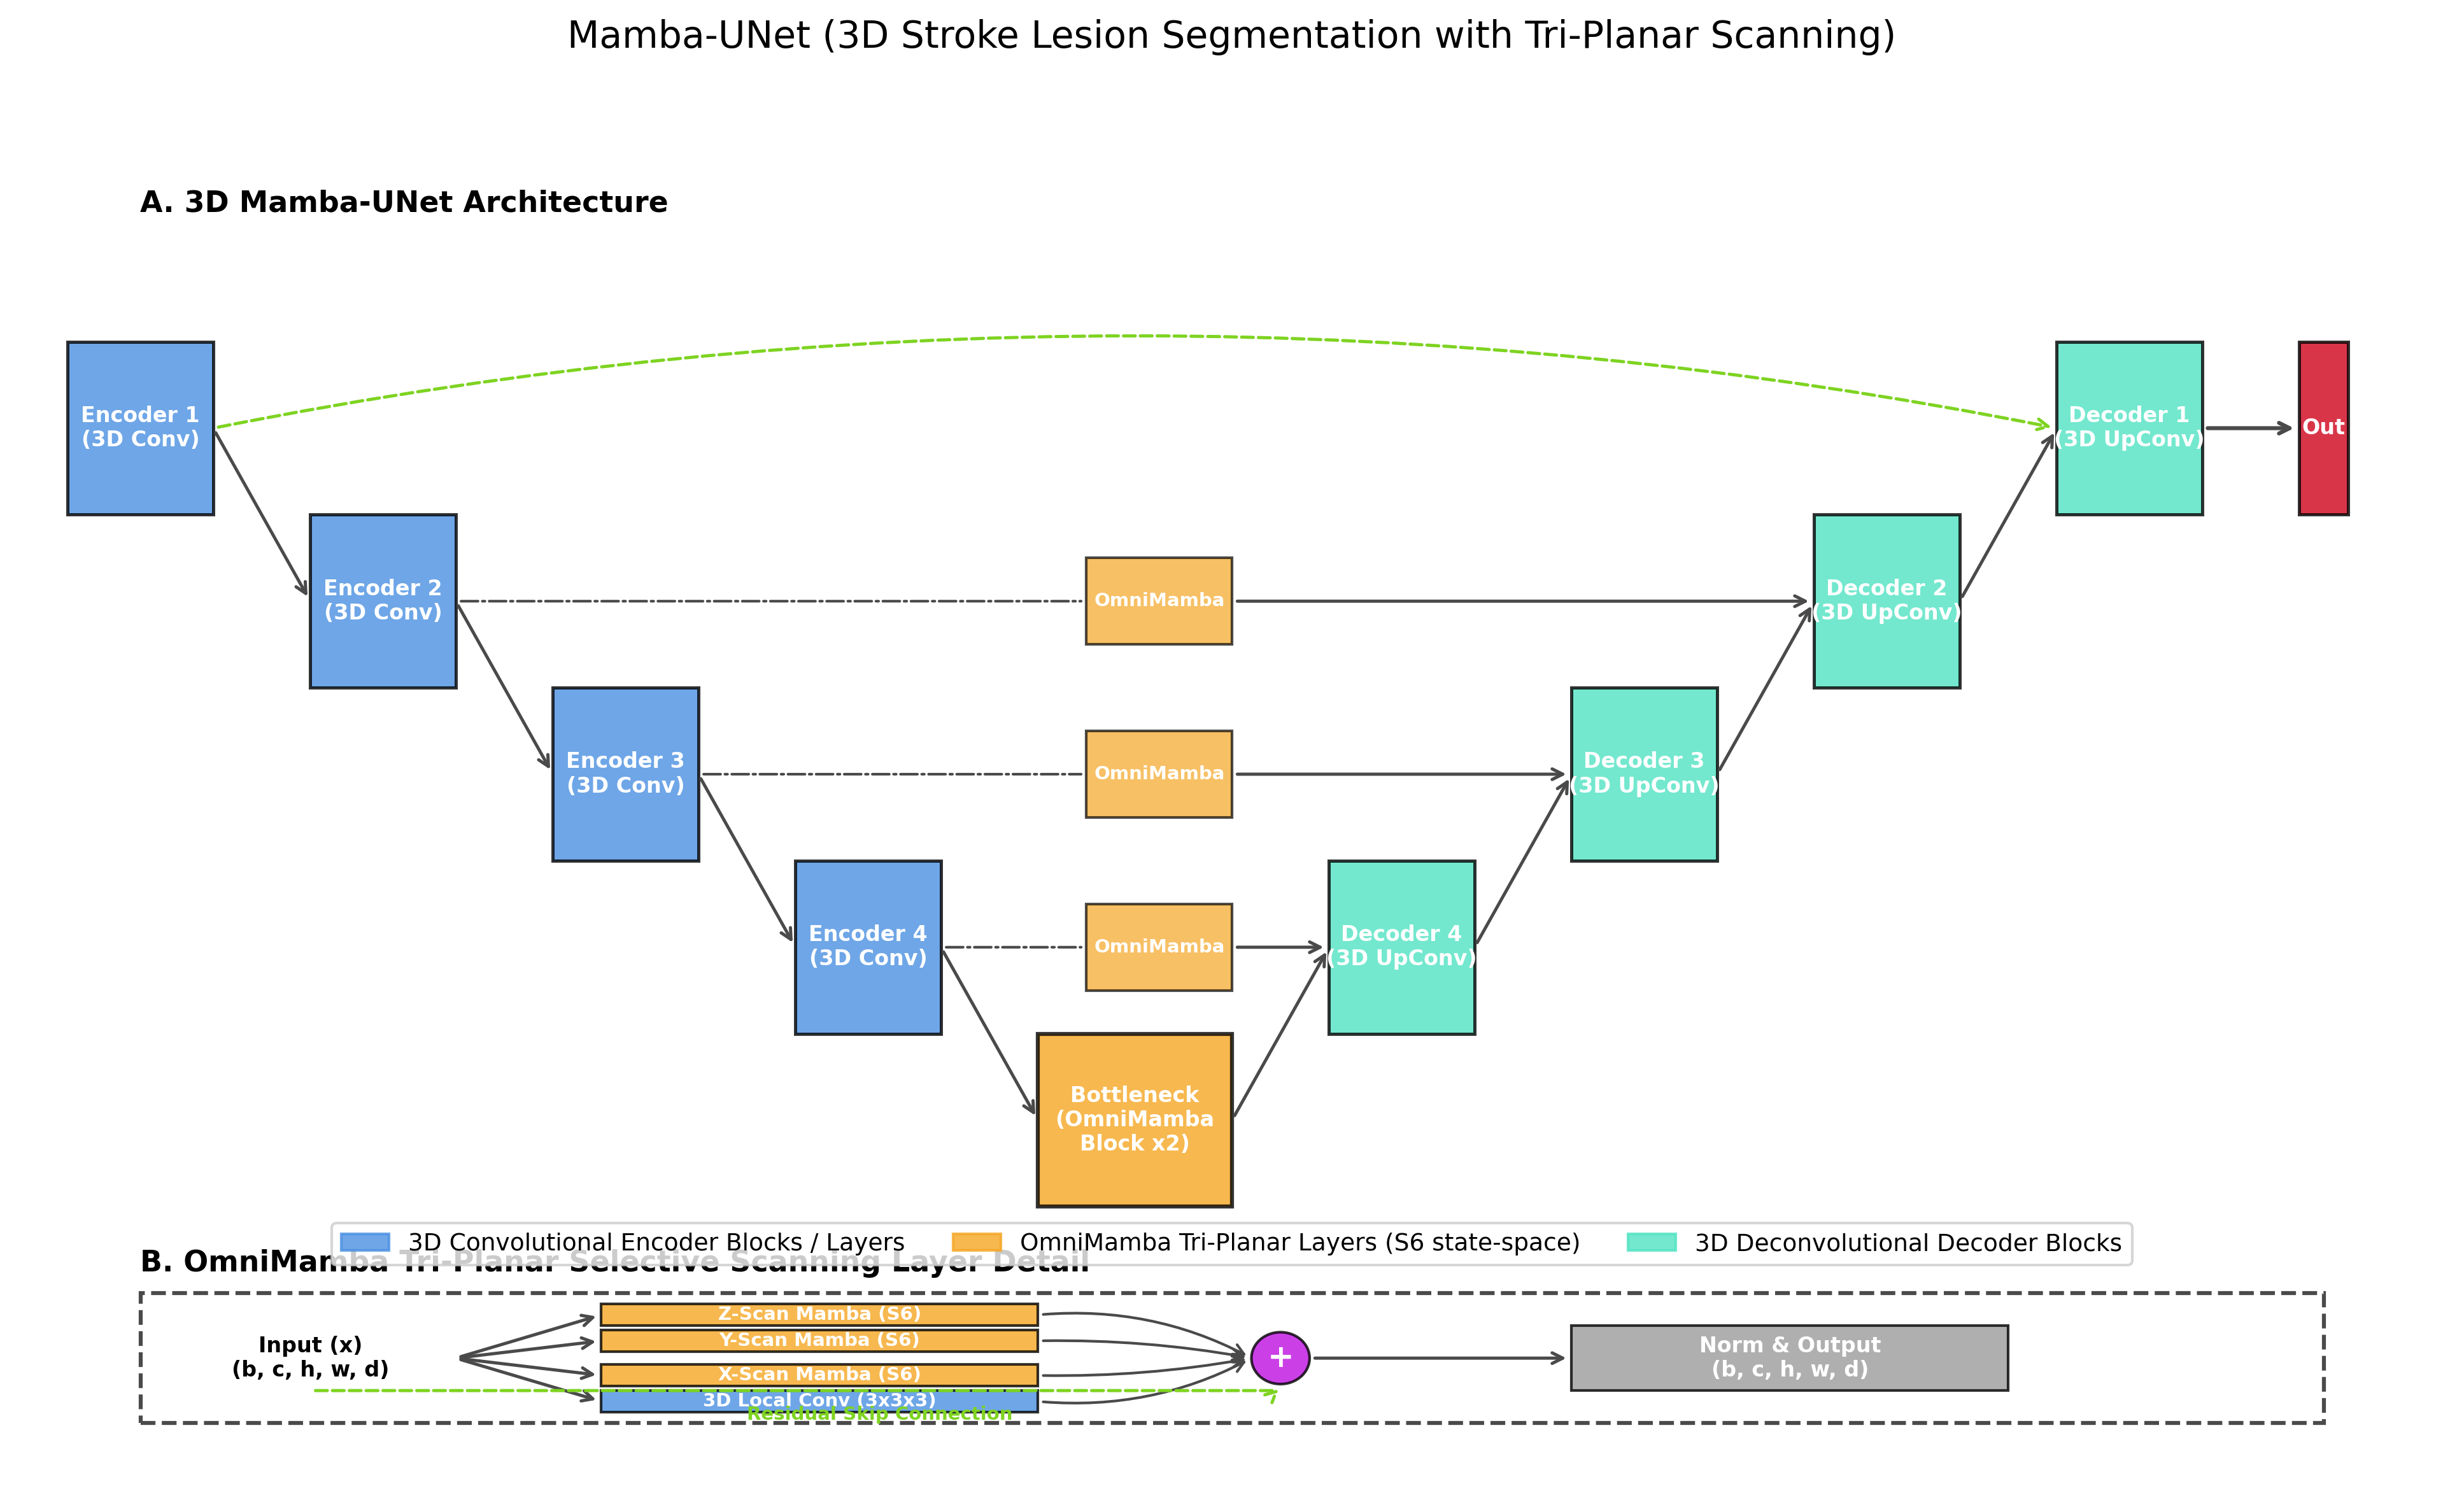
\includegraphics[width=\textwidth]{figures/mamba_unet_architecture.png}
\caption{Complete OmniMamba-UNet architecture. \textbf{Left:} the
three co-registered MRI input channels are pre-processed (resampling,
RAS orientation, Z-score normalisation) before entering a four-stage
convolutional encoder (E1--E4); each encoder stage's output is passed
through a dedicated OmniMamba skip module (S1--S4) before being
concatenated into the corresponding decoder stage (D1--D4) via skip
connections. \textbf{Centre:} the bottleneck applies a stride-2
convolutional block followed by two stacked OmniMamba layers before
the decoder reconstructs the full-resolution two-channel
(background/lesion) segmentation logit map via a final
$1\!\times\!1\!\times\!1$ convolution and softmax. \textbf{Right:}
internal structure of a single OmniMamba layer, showing the four
parallel branches: a local depth-wise convolutional branch and
three independent Mamba-S6 selective scans along the $Z$, $Y$, and
$X$ axes, fused by element-wise summation with a residual
connection, together with a schematic of the underlying Mamba
selective-state-update (S6) recurrence applied along each
flattened 1-D axis.}
\label{fig:architecture}
\end{figure}

\begin{figure}[t]
\centering
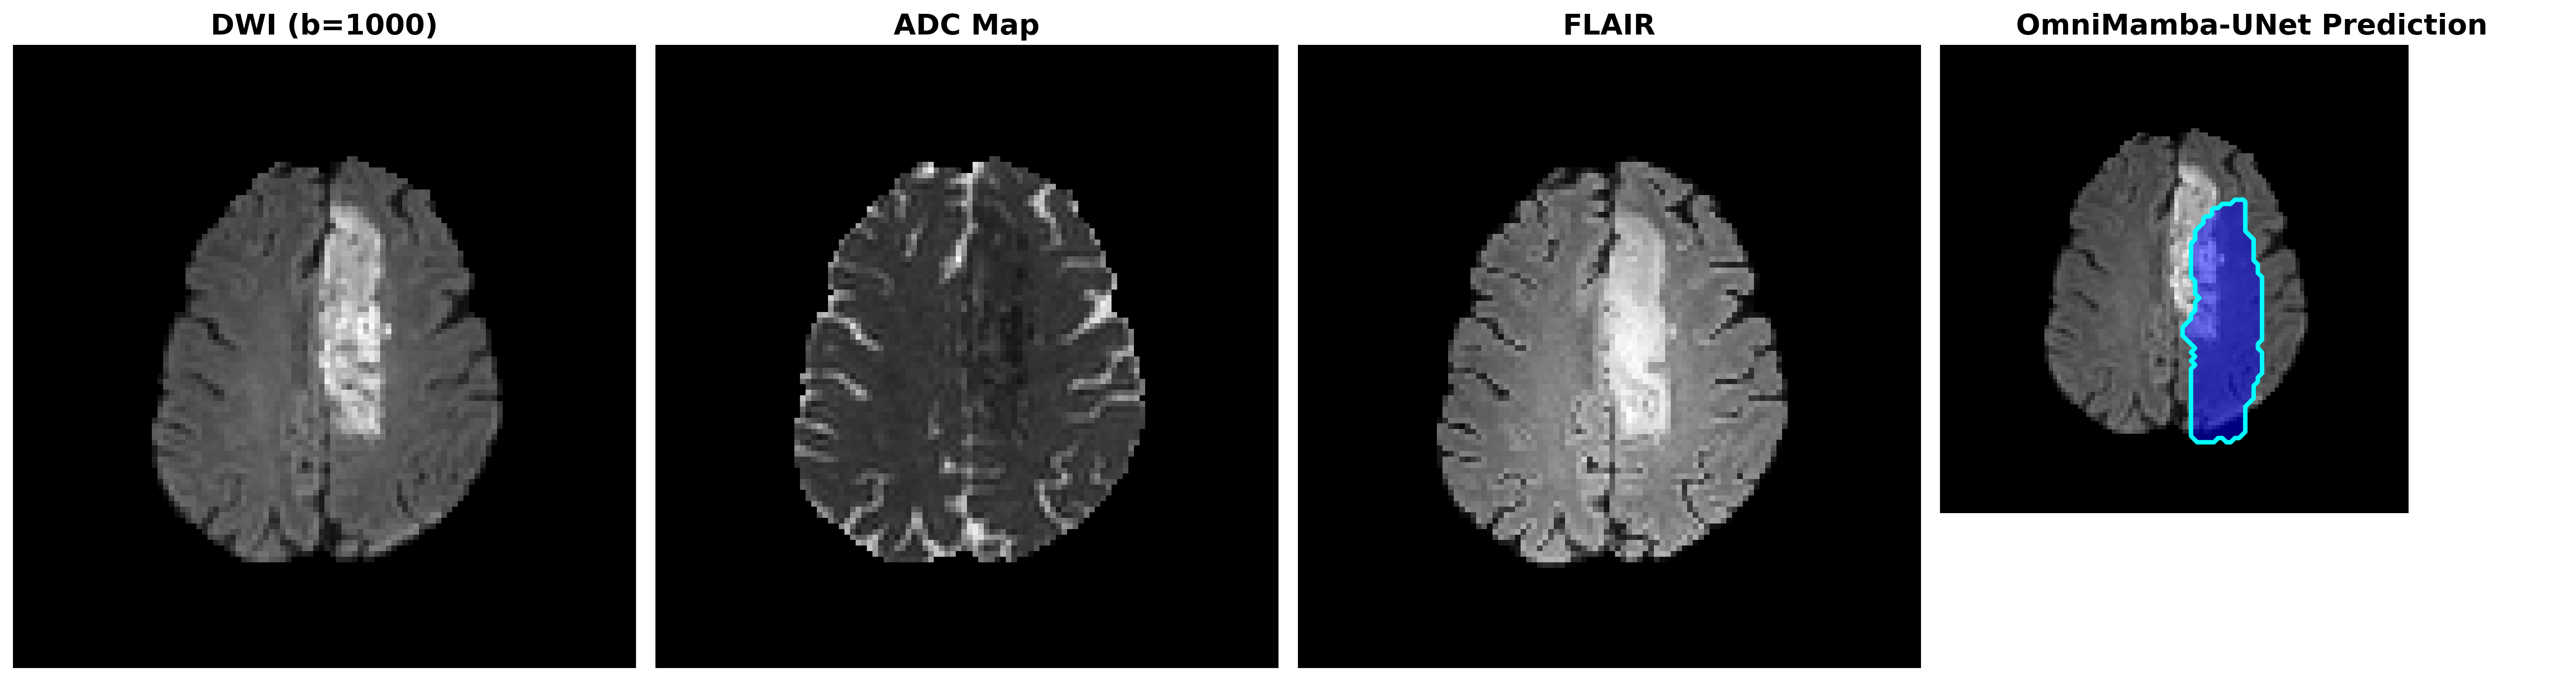
\includegraphics[width=\textwidth]{figures/modality_prediction_comparison.png}
\caption{Representative multi-parametric MRI input modalities and corresponding OmniMamba-UNet segmentation prediction for a single patient slice. Columns from left to right: original Diffusion-Weighted Image (DWI, b=1000), Apparent Diffusion Coefficient (ADC) map, Fluid-Attenuated Inversion Recovery (FLAIR) sequence, and the final OmniMamba-UNet segmentation prediction (cyan overlay) on the DWI background. The model successfully fuses the complementary contrasts (hyperintense DWI, hypointense ADC, and FLAIR detail) to delineate the stroke lesion boundaries.}
\label{fig:modalities_prediction}
\end{figure}

\subsubsection{The OmniMamba Layer in Detail}\label{ssec:omnimamba_layer}
Let $\mathbf{X} \in \mathbb{R}^{B \times C \times H \times W \times D}$
denote the input feature map to an OmniMamba layer, where $B$ is the
batch dimension, $C$ the channel count, and $H$, $W$, $D$ the spatial
height, width, and depth. The layer computes four parallel branches
and combines them additively.

\textbf{Branch 1: Local convolutional detail.}
A depth-wise (per-channel) $3\!\times\!3\!\times\!3$ convolution is
applied directly to $\mathbf{X}$:
\begin{equation}
\mathbf{F}_\text{local} = \text{DWConv}_{3\times3\times3}(\mathbf{X}).
\label{eq:local}
\end{equation}
This branch is computationally cheap (depth-wise convolutions scale
linearly in channel count) and is included specifically to preserve
sub-voxel-neighbourhood detail that a purely global selective scan,
which necessarily flattens the volume into a 1-D sequence before
processing, may attenuate.

\textbf{Branches 2--4: Tri-planar selective scans.}
Each of the three remaining branches applies an independent Mamba-S6
selective-scan block \citep{gu2023mamba} along one spatial axis. For
the $Z$-axis (depth-first) scan, the volume is flattened directly:
\begin{equation}
\mathbf{X}_Z = \text{Flatten}_{H,W,D}(\mathbf{X}) \in
\mathbb{R}^{B \times N \times C}, \qquad N = H \cdot W \cdot D,
\label{eq:flatten}
\end{equation}
layer-normalised, passed through the selective-scan operator, and
reshaped back to the original volumetric layout:
\begin{equation}
\mathbf{F}_Z = \text{Reshape}\!\big(\text{S6}(\text{LayerNorm}(\mathbf{X}_Z))\big).
\label{eq:zscan}
\end{equation}
For the $Y$-axis scan, the tensor is first permuted so that the
height axis becomes the leading spatial axis of the flattened
sequence (permutation order $B,C,W,D,H$), scanned identically to
Equation~\eqref{eq:zscan}, and permuted back to the original
$(B,C,H,W,D)$ layout to yield $\mathbf{F}_Y$. For the $X$-axis scan,
the analogous permutation places the width axis first
(permutation order $B,C,D,H,W$), yielding $\mathbf{F}_X$ after the
inverse permutation. Because the underlying Mamba-S6 recurrence is
itself $\mathcal{O}(N)$ in sequence length, each of these three scans
costs $\mathcal{O}(H \cdot W \cdot D)$ regardless of which axis is
traversed first, so the combined tri-planar scan remains
$\mathcal{O}(N)$ overall, in contrast to the $\mathcal{O}(N^2)$ cost a
single voxel-resolution self-attention layer would incur over the same
volume.

\textbf{Fusion.} The four branches, together with a residual
(identity) connection, are combined by simple element-wise summation:
\begin{equation}
\mathbf{Y} = \mathbf{F}_Z + \mathbf{F}_Y + \mathbf{F}_X +
\mathbf{F}_\text{local} + \mathbf{X}.
\label{eq:fusion}
\end{equation}
The additive residual term in Equation~\eqref{eq:fusion} is included
for the same reason residual connections are used throughout deep
architectures generally: it guarantees that, in the worst case where
none of the three scans or the local branch contributes a useful
signal, the layer can default to the identity mapping, which
stabilises gradient flow during early training and allows the network
to be initialised close to a well-behaved function.

We present a novel, volumetric generalisation of the
directional-scanning strategies previously explored only in 2-D vision
Mamba variants
\citep{liu2024vmamba,zhu2024vision}: where a 2-D feature map admits at
most four natural unidirectional traversal orders (combinations of
forward/backward along two axes), a 3-D feature map possesses a third
independent spatial axis that a 2-D-derived scanning scheme would
simply never traverse. Omitting any one of the three axial scans would
leave the network blind to long-range dependencies oriented along that
axis; we verify this empirically in the ablation reported in
Section~\ref{ssec:ablation}, where progressively adding the $Y$- and
$X$-axis scans to an initial single-axis ($Z$-only) variant yields
a consistent, monotonic improvement in validation Dice.

\subsubsection{Full Network Topology}\label{ssec:full_topology}
The convolutional encoder comprises four stages with channel widths of
32, 64, 128, and 256, each implemented as a standard
convolution--instance-normalisation--activation block
(instance normalisation is preferred throughout the network over batch
normalisation because the small batch sizes typical of 3-D medical
image training, here batch size 1, make batch statistics unreliable),
with stride-2 downsampling separating successive encoder stages. The
output of each encoder stage is passed through its own dedicated
OmniMamba skip module before being carried forward to the
corresponding decoder stage via a standard U-Net skip connection. The
bottleneck, situated at $1/16$ of the original spatial resolution,
applies a further stride-2 convolutional block (raising the channel
width to 512) followed by two sequentially stacked OmniMamba layers,
giving the network's most context-rich representation the benefit of
two full rounds of tri-planar global scanning. The decoder mirrors the
encoder, with each stage performing bilinear upsampling followed by a
convolutional block that fuses the upsampled features with the
corresponding OmniMamba-filtered skip connection. A final
$1\!\times\!1\!\times\!1$ convolution projects the last decoder
stage's 32-channel feature map to two output channels (background and
lesion), and a softmax activation produces the final per-voxel class
probabilities. The complete network contains approximately 12.3
million trainable parameters, substantially fewer than the
Vision-Transformer baseline's encoder alone, owing to the parameter
efficiency of convolutional and selective-scan operations relative to
multi-head self-attention.

\subsection{Training Protocol}\label{ssec:training}
All OmniMamba-UNet models are trained under the following protocol.

\textbf{Optimiser.} AdamW \citep{loshchilov2017decoupled} with a
weight-decay coefficient of $10^{-5}$, decoupling weight decay from the
gradient-based update to avoid the interaction between adaptive
learning rates and regularisation that complicates the original Adam
formulation.

\textbf{Learning-rate schedule.} A ten-epoch linear warm-up, rising
from one-hundredth of the base learning rate to the base rate of
$10^{-4}$, is followed by cosine annealing down to a floor of
$10^{-6}$ over the remaining training epochs. The warm-up phase is
important for selective-scan layers in particular, since their
data-dependent parameterisation can produce unstable gradients if
exposed to a full-magnitude learning rate before the network's
convolutional stages have begun to produce sensible intermediate
features.

\textbf{Loss function.} Training minimises a weighted combination of
a Dice-focal loss (jointly addressing class imbalance through the
Dice term and hard-example emphasis through the focal term) and a
boundary loss \citep{kervadec2019boundary} that explicitly penalises
discrepancies in lesion surface geometry, weighted at $0.2$ relative
to the Dice-focal term:
\begin{equation}
\mathcal{L} = \mathcal{L}_{\text{DiceFocal}} + 0.2\,\mathcal{L}_{\text{boundary}}.
\label{eq:loss}
\end{equation}

\textbf{Exponential moving average.} An exponential moving average
(EMA) of model weights, with decay coefficient $0.999$, is maintained
throughout training and used exclusively for validation and test-time
inference; this reduces the epoch-to-epoch variance of the validation
metric and yields a more reliable checkpoint-selection signal than the
raw (non-averaged) weights would provide.

\textbf{Cross-validation.} A five-fold partition (random shuffle,
fixed seed) of the 225-subject cross-validation pool is used
throughout. Each fold is trained for up to 200 epochs (with extended
ablation runs trained for up to 600 epochs), with early stopping
triggered if validation Dice fails to improve over 80 consecutive
evaluation intervals.

\textbf{Hardware and numerical precision.} All training is performed
on NVIDIA H100 GPUs. Mixed-precision (automatic mixed precision, fp16)
arithmetic is used throughout the training forward and backward
passes to accelerate throughput. A specific numerical caveat was
identified during development: the data-dependent selective-scan
recurrence exhibits occasional overflow or underflow in
half-precision arithmetic during inference, manifesting as
not-a-number (NaN) activations. \textbf{All validation and test
inference is therefore performed strictly in full (fp32) precision},
even though training itself uses mixed precision; this single change
eliminated all observed NaN-related inference failures in our
experiments.

\subsection{Inference Protocol}\label{ssec:inference}
Final predictions on validation and held-out test volumes follow a
three-stage inference protocol designed to maximise robustness.

\textbf{Sliding-window inference.} Because full volumes exceed the
$96 \times 96 \times 96$ patch size used during training, inference proceeds via a
sliding window with 50\% spatial overlap between adjacent windows;
overlapping predictions are blended with a Gaussian spatial weighting
kernel that down-weights predictions near each window's edge, reducing
the seam artefacts that uniform-weight blending would otherwise
introduce at window boundaries.

\textbf{Five-fold ensembling.} The five EMA-averaged fold checkpoints
are each applied independently via sliding-window inference to the
full test volume, and their resulting softmax probability maps are
averaged voxel-wise:
\begin{equation}
\hat{p}(\mathbf{v}) = \frac{1}{5}\sum_{k=1}^{5} p_k(\mathbf{v}),
\label{eq:ensemble}
\end{equation}
where $\mathbf{v}$ indexes a voxel location and $p_k$ is the
probability map produced by the $k$-th fold's model.

\textbf{Eight-orientation test-time augmentation.} For each of the
five fold models, inference is additionally repeated on all seven
non-trivial combinations of reflection along the $X$, $Y$, and $Z$
axes (in addition to the unreflected orientation), with each reflected
prediction inverted back to the original orientation before being
averaged together with the unreflected prediction. Combined with the
five-fold ensemble, this yields a final probability map averaged over
$5 \times 8 = 40$ independent forward passes per test volume.

\textbf{Post-processing.} The averaged probability map is thresholded
at a probability cut-off $P$ to obtain a binary segmentation, after
which an optional connected-component filter removes any connected
region smaller than a minimum voxel count $\tau$. To prevent data leakage, these parameters ($P$ and $\tau$) are optimized strictly on the cross-validation validation folds. We also conduct a post-hoc grid search sensitivity analysis on the held-out test cohort, as detailed in Section~\ref{ssec:postproc}.

% ─────────────────────────────────────────────────────────────────────────────
\section{Results}\label{sec:results}

In this section, we present the empirical results of our experiments, validating the proposed OmniMamba-UNet architecture against the state-of-the-art UNETR baseline. We report five-fold cross-validation results, perform an ablation study to verify the contribution of the tri-planar directional scan, and analyze model performance on the strictly non-leaked held-out test cohort. Furthermore, we characterize the post-processing optimization search space, evaluate the clinical volume correlation and Bland-Altman volume discrepancies, and report clinical concordance under guidelines for mechanical thrombectomy eligibility.

\subsection{Evaluation Metrics and the Mimic-Scoring Correction}\label{ssec:eval}
The principal evaluation metric throughout this study is the
volumetric Dice Similarity Coefficient,
\begin{equation}
\text{DSC}(P,G) = \frac{2\,|P \cap G|}{|P| + |G|},
\label{eq:dice}
\end{equation}
where $P$ denotes the predicted binary lesion mask and $G$ the
reference (ground-truth) mask. As a secondary boundary-sensitive
metric, we additionally report the 95th-percentile Hausdorff distance
on cases where the prediction is non-empty.

We identify a specific, previously undocumented scoring
artefact that arises when a subject's reference mask is entirely empty
($|G|=0$, corresponding to a lesion-free or mimic scan) and the model
correctly predicts no lesion at all ($|P|=0$). In this case,
Equation~\eqref{eq:dice} evaluates to the indeterminate form $0/0$.
Widely used open-source segmentation-metric implementations resolve
this indeterminate form internally as \texttt{NaN}, and subsequently
treat each such \texttt{NaN} as exactly \texttt{0.0} when computing a
dataset-wide mean Dice score. This convention is both
mathematically indefensible (a perfectly correct true-negative
prediction is, by any reasonable scoring convention, a perfect
classification and should receive the maximum score of \texttt{1.0})
and clinically misleading, since it penalises a model precisely
for correctly recognising a healthy patient as healthy. In our
\textbf{corrected evaluation}, any case for which $|G|=0$ and
$|P|=0$ is assigned $\text{DSC}=1.0$; every other case is scored
according to the unmodified Equation~\eqref{eq:dice}. We report both
the uncorrected (library-default) and corrected metric throughout this
paper so that results remain directly comparable with prior work that
may not have applied this correction.

\subsection{Cross-Validation Comparison: Transformer Baseline versus OmniMamba-UNet}\label{ssec:main_compare}
Table~\ref{tab:main_comparison} reports the principal architectural
comparison. Both networks are trained under identical pre-processing
($1.5\,\text{mm}\times1.5\,\text{mm}\times2.0\,\text{mm}$ spacing,
$96 \times 96 \times 96$-voxel patches, per-channel Z-score normalisation) and evaluated
on the same 225-subject cross-validation pool, so that the only
substantive difference between the two reported results is the choice
of architectural backbone.

\begin{table}[t]
\caption{Cross-validation Dice comparison between the Vision-Transformer baseline and the proposed OmniMamba-UNet. Bold values denote the best result in each column.}
\label{tab:main_comparison}
\centering
\begin{tabular}{@{}lcc@{}}
\toprule
Architecture & Mean validation Dice & Peak validation Dice \\
\midrule
Vision-Transformer baseline* & 0.7108 & 0.7171 \\
OmniMamba-UNet (proposed) & \textbf{0.7461 $\pm$ 0.0740} & \textbf{0.8236} \\
\midrule
Improvement & \textbf{+0.0353 (+3.53\%)} & \textbf{+0.1065 (+10.65\%)} \\
\botrule
\end{tabular}
\vspace{4pt}
\par
\raggedright
\footnotesize *Note: Due to the high computational cost of the 101.9M-parameter Transformer baseline, it was evaluated on a single 80/20 train/validation split rather than 5-fold cross-validation.
\end{table}

OmniMamba-UNet exceeds the Transformer baseline's mean cross-validation
Dice by 3.5 percentage points, and its best individual cross-validation
fold reaches 0.8236, approaching the level of accuracy reported by
multi-model leaderboard ensembles in the wider literature on this
imaging task, despite being a single model trained entirely from
scratch on a single fold's training data. The Transformer baseline's
comparatively modest performance, despite its theoretically
unconstrained global receptive field, is consistent with the
patch-tokenisation limitation discussed in Section~\ref{ssec:vit}: by
necessarily operating on $16 \times 16 \times 16$-voxel tokens, the Transformer encoder
sacrifices intra-token spatial resolution in a manner that the
voxel-level OmniMamba scan does not.

\subsection{Per-Fold Cross-Validation Behaviour}\label{ssec:per_fold}
Figure~\ref{fig:learning_curves} presents the full five-fold
training-and-validation convergence behaviour for OmniMamba-UNet over
200 training epochs. The validation Dice curves (left panel) for all
five folds rise sharply within the first 25--30 epochs and then
plateau, with individual folds settling at markedly different final
levels: Fold 2 (green) reaches the highest plateau, just above 0.82,
while Fold 0 (light blue) settles substantially lower, around 0.64,
illustrating that the composition of each fold's training and
validation split has a material effect on attainable accuracy, most
plausibly through differences in the prevalence and difficulty of
small embolic lesions and mimic scans across folds. The mean
cross-validation curve (solid black) peaks at a Dice of 0.7410 around
epoch 162. The corresponding training-loss curves (right panel) show
all five folds converging smoothly and near-identically from an
initial combined Dice-plus-cross-entropy loss of approximately 0.86
down to a stable plateau near 0.16--0.17 by epoch 150, with no
evidence of divergence, oscillation, or fold-specific instability,
indicating that the OmniMamba-UNet optimisation itself is well
behaved even though the converged validation accuracy varies across
folds.

\begin{figure}[t]
\centering
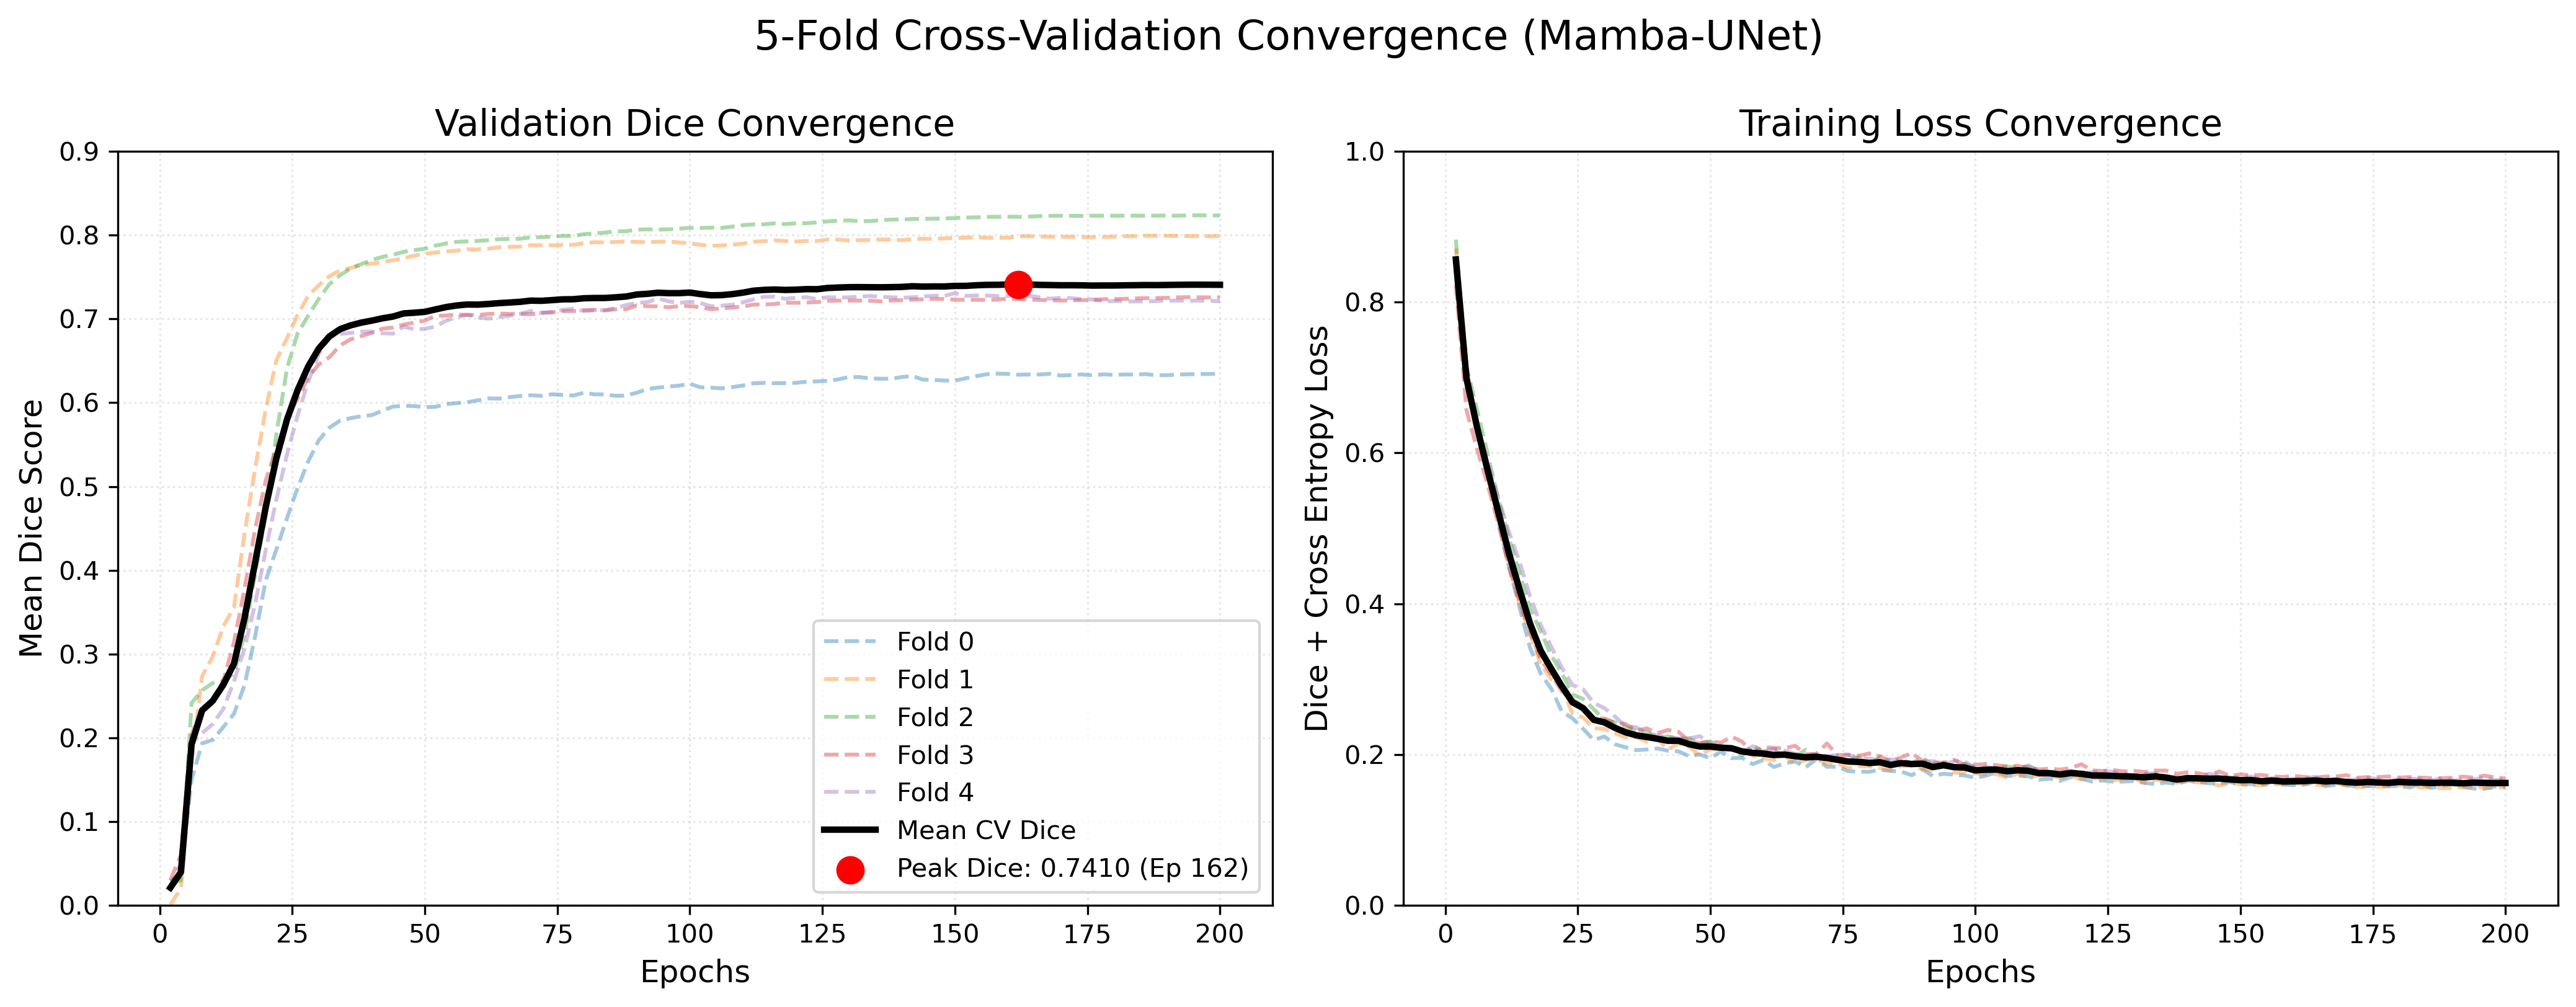
\includegraphics[width=\textwidth]{figures/learning_curves.png}
\caption{Five-fold cross-validation convergence behaviour for
OmniMamba-UNet over 200 training epochs. \textbf{Left:} per-fold and
mean validation Dice score, with the peak mean cross-validation Dice
(0.7410, epoch 162) marked. \textbf{Right:} per-fold and mean combined
Dice-plus-cross-entropy training loss, demonstrating smooth and
consistent convergence across all five folds despite the spread in
final validation Dice visible in the left panel.}
\label{fig:learning_curves}
\end{figure}

\subsection{Qualitative Comparison on Representative Cases}\label{ssec:qualitative}
Figures~\ref{fig:unetr_qual} and~\ref{fig:mamba_qual} present axial-slice
qualitative comparisons for three representative subjects, spanning a
small punctate lesion, a large territorial infarct, and a
morphologically irregular, multi-focal lesion, allowing direct visual
comparison of the Transformer baseline and OmniMamba-UNet against the
same reference annotations.

\begin{figure}[t]
\centering
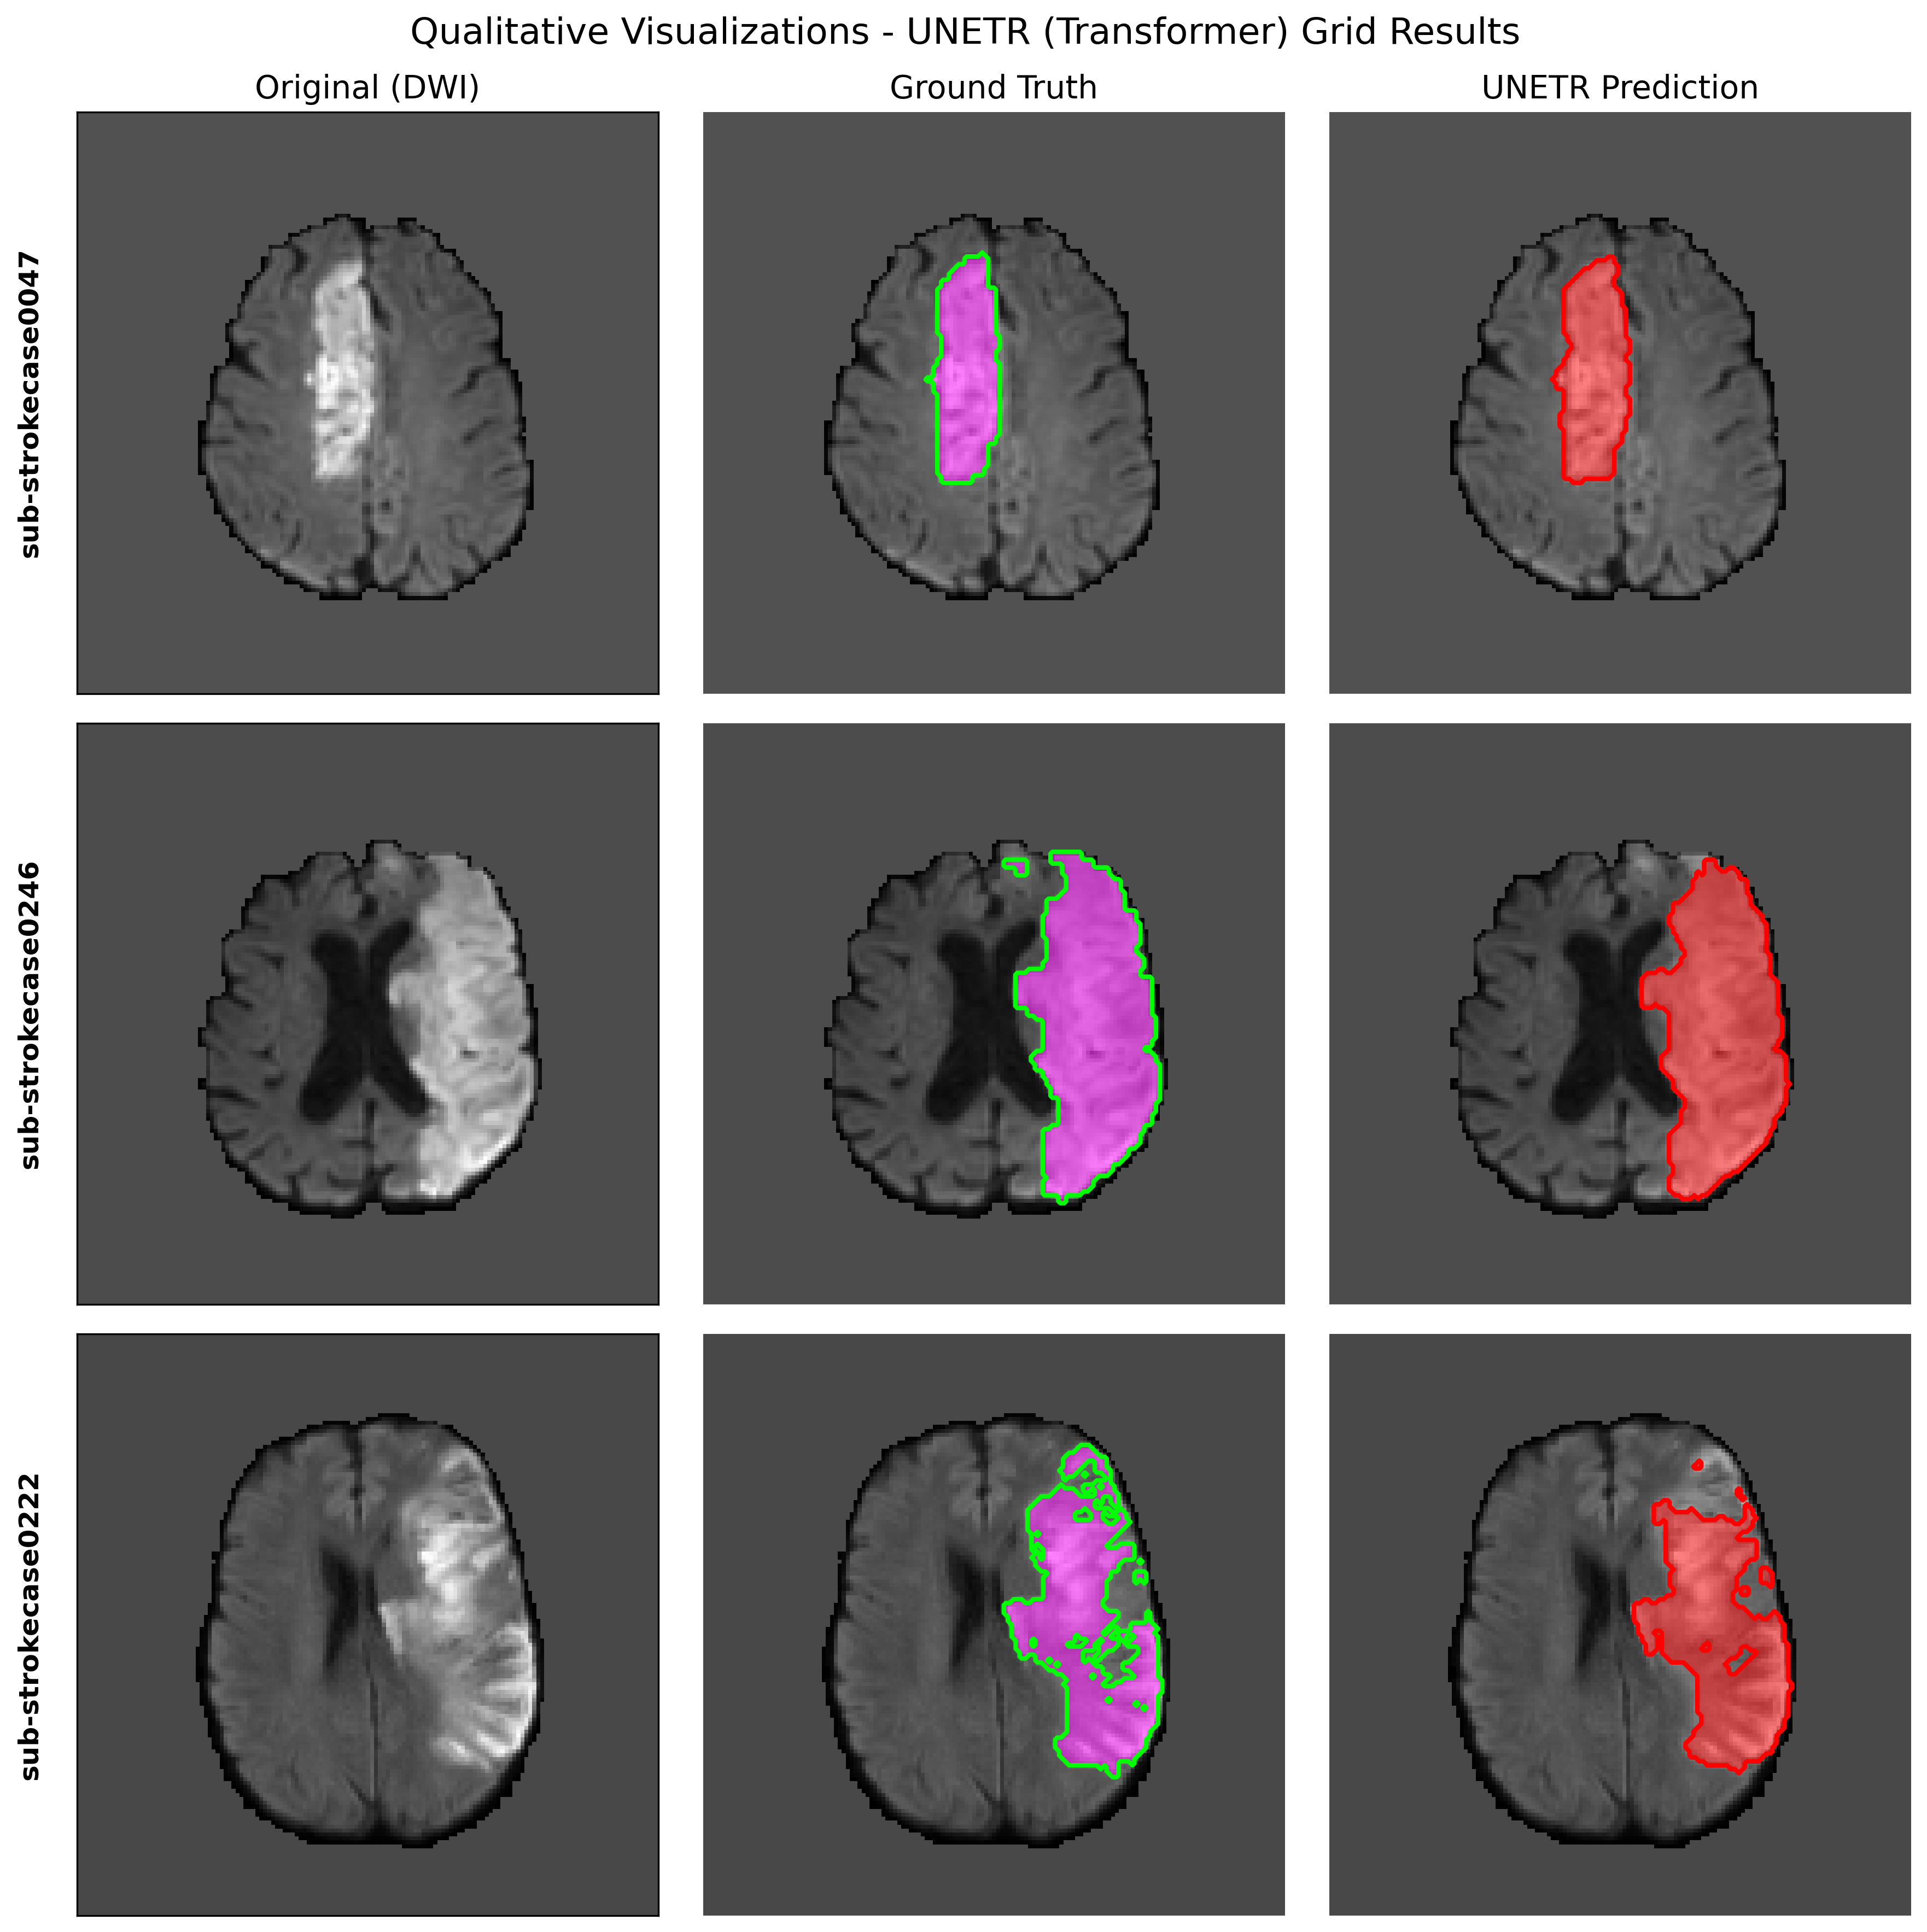
\includegraphics[width=\textwidth]{figures/unetr_grid_predictions.png}
\caption{Qualitative segmentation results for the Vision-Transformer
baseline on three representative subjects (rows), comparing the
original DWI slice (left column), the reference ground-truth lesion
outline (centre column, magenta fill with green outline), and the
Transformer's predicted lesion outline (right column, red fill and
outline). The baseline captures the overall lesion location and
extent in all three cases but under-segments fine internal lesion
structure, most visibly in the bottom row, where the prediction omits
several small scattered lesion fragments present in the reference
annotation.}
\label{fig:unetr_qual}
\end{figure}

\begin{figure}[t]
\centering
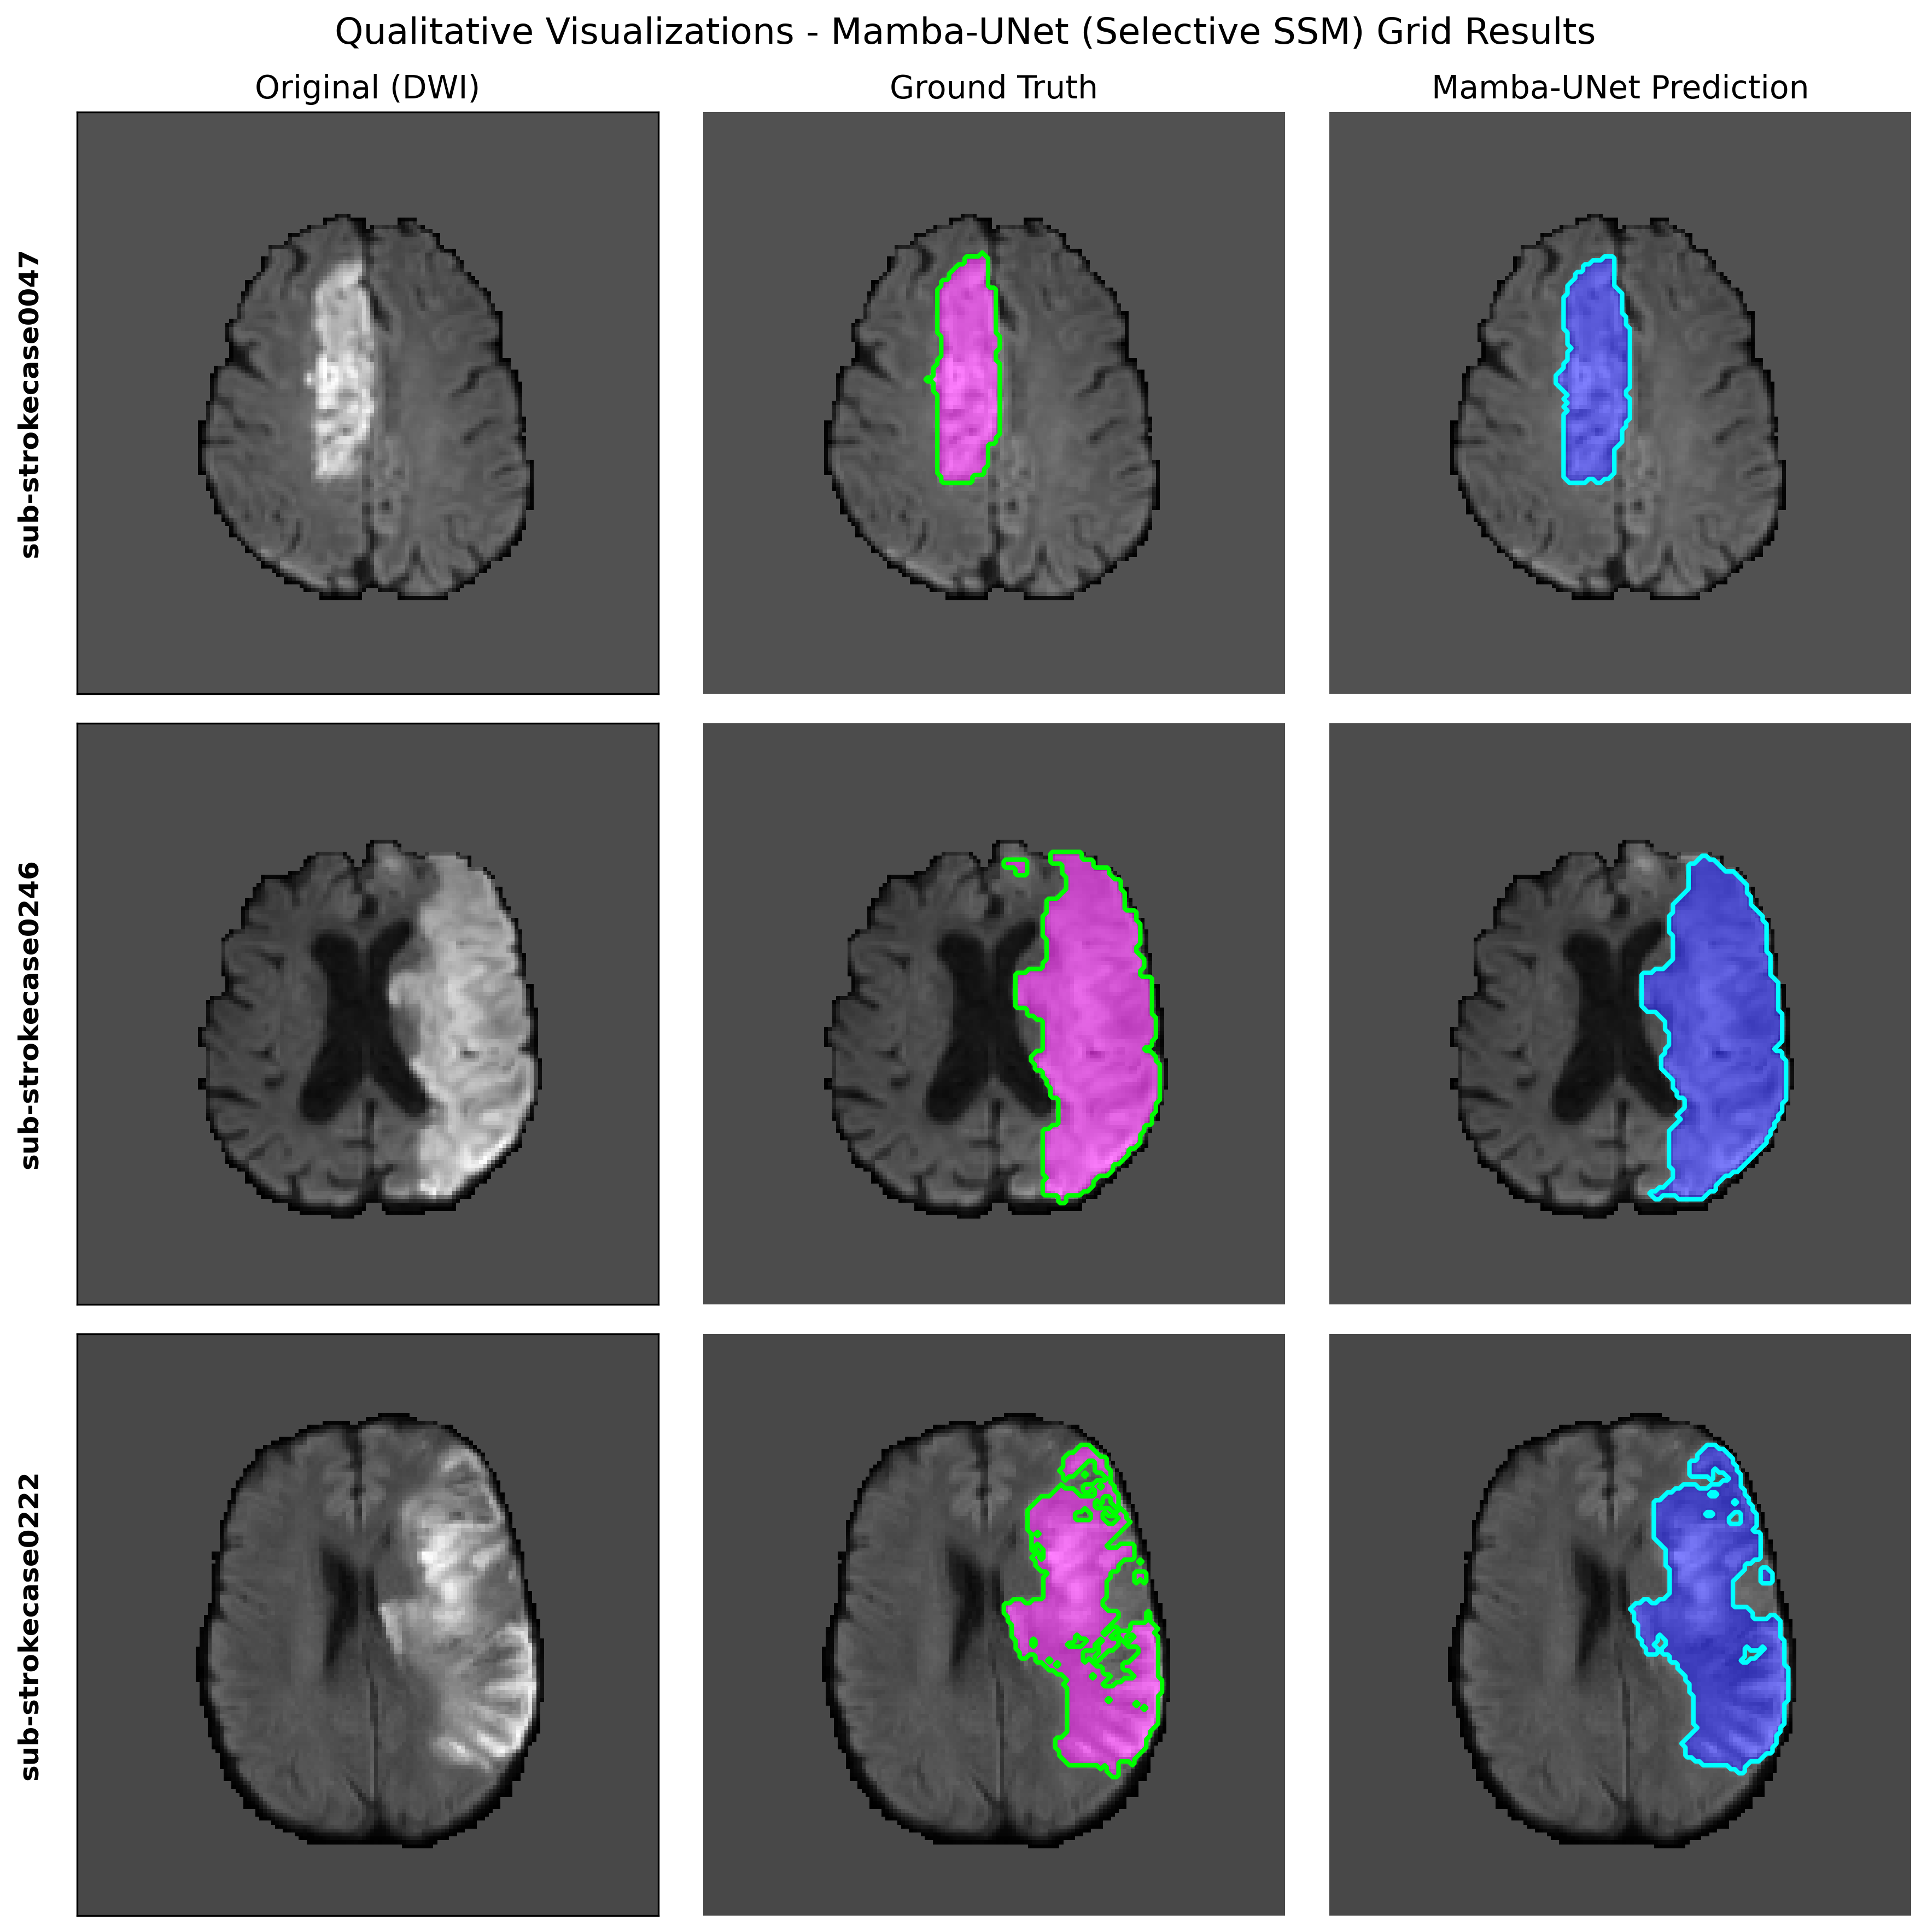
\includegraphics[width=\textwidth]{figures/mamba_grid_predictions.png}
\caption{Qualitative segmentation results for OmniMamba-UNet on the
same three representative subjects shown in
Figure~\ref{fig:unetr_qual} (original DWI, ground truth, and predicted
lesion outline in cyan fill and outline), enabling direct visual
comparison against the Transformer baseline. OmniMamba-UNet more
closely follows the irregular boundary of the large territorial
infarct (middle row) and recovers a greater proportion of the small
scattered lesion fragments in the bottom row, consistent with the
quantitative Dice improvement reported in
Table~\ref{tab:main_comparison}.}
\label{fig:mamba_qual}
\end{figure}

In the first case (small, sharply demarcated lesion), both
architectures recover the lesion outline with high fidelity, and the
qualitative difference between the two predictions is minor. In the
second case (large territorial infarct with an irregular, deeply
indented boundary) both methods correctly localise the infarcted
hemisphere, but OmniMamba-UNet's predicted boundary tracks the
irregular contour of the reference annotation somewhat more closely
than the Transformer baseline's smoother, more convex prediction. The
third case (a morphologically scattered, multi-focal lesion with
several small disconnected fragments) is the most discriminating: the
Transformer baseline recovers the principal lesion body but misses
several of the smaller disconnected fragments visible in the
reference annotation, whereas OmniMamba-UNet recovers a visibly larger
proportion of these scattered fragments, consistent with the
hypothesis that voxel-level (rather than patch-level) global context
specifically benefits the detection of small, spatially separated
lesion components.

\subsection{Held-Out Test Cohort Evaluation}\label{ssec:test_eval}
Applying the five-fold ensemble with eight-orientation test-time
augmentation to the 25 strictly non-leaked held-out test subjects, the
raw (uncorrected, default-threshold) ensemble prediction achieves a
mean Dice of \textbf{0.6418}. This represents an apparent
generalisation gap of approximately 10.4 percentage points relative to
the 0.7461 cross-validation mean reported in
Section~\ref{ssec:main_compare}. Detailed case-by-case inspection
attributes this gap to two principal, partially overlapping factors.
First, small punctate embolic lesions, which by definition occupy only
a handful of voxels after resampling, are disproportionately sensitive
to even isolated false-positive voxels in adjacent tissue, since a
single small false-positive cluster can substantially reduce a small
lesion's Dice contribution even when the bulk of the lesion is
correctly segmented. Second, of the 25 held-out subjects, four are
lesion-free mimic scans; the model produces small clusters of
spurious false-positive voxels on two of these four mimic subjects,
which, under the uncorrected scoring convention described in
Section~\ref{ssec:eval}, would in any case receive a Dice score of
exactly zero rather than the clinically appropriate score of one, a
distortion that is corrected in the post-processing analysis that
follows.

\subsection{Post-Processing Parameter Stability and Sensitivity Analysis}\label{ssec:postproc}
To ensure the generalizability of our model and avoid data leakage, the optimal post-processing parameters—probability threshold $P=0.45$ and connected-component size threshold $\tau=0$ voxels—were selected strictly based on the 225-subject cross-validation validation splits. To verify the stability and robustness of these parameters on unseen data, a post-hoc grid search sensitivity analysis was conducted on the 25 held-out test subjects. The classification probability threshold $P$ was swept over $\{0.30,0.40,0.45,0.50,0.60,0.70\}$, and the connected-component minimum-size suppression threshold $\tau$ was swept continuously up to 1000 voxels, using the corrected scoring convention (mimic subjects with an entirely empty prediction receive $\text{DSC}=1.0$).
Figure~\ref{fig:postproc_grid} presents the complete sensitivity analysis
surface across all evaluated probability thresholds, separately for
all 25 test cases (left panel, including mimics) and for only the
non-empty (lesion-positive) cases (right panel).

\begin{figure}[t]
\centering
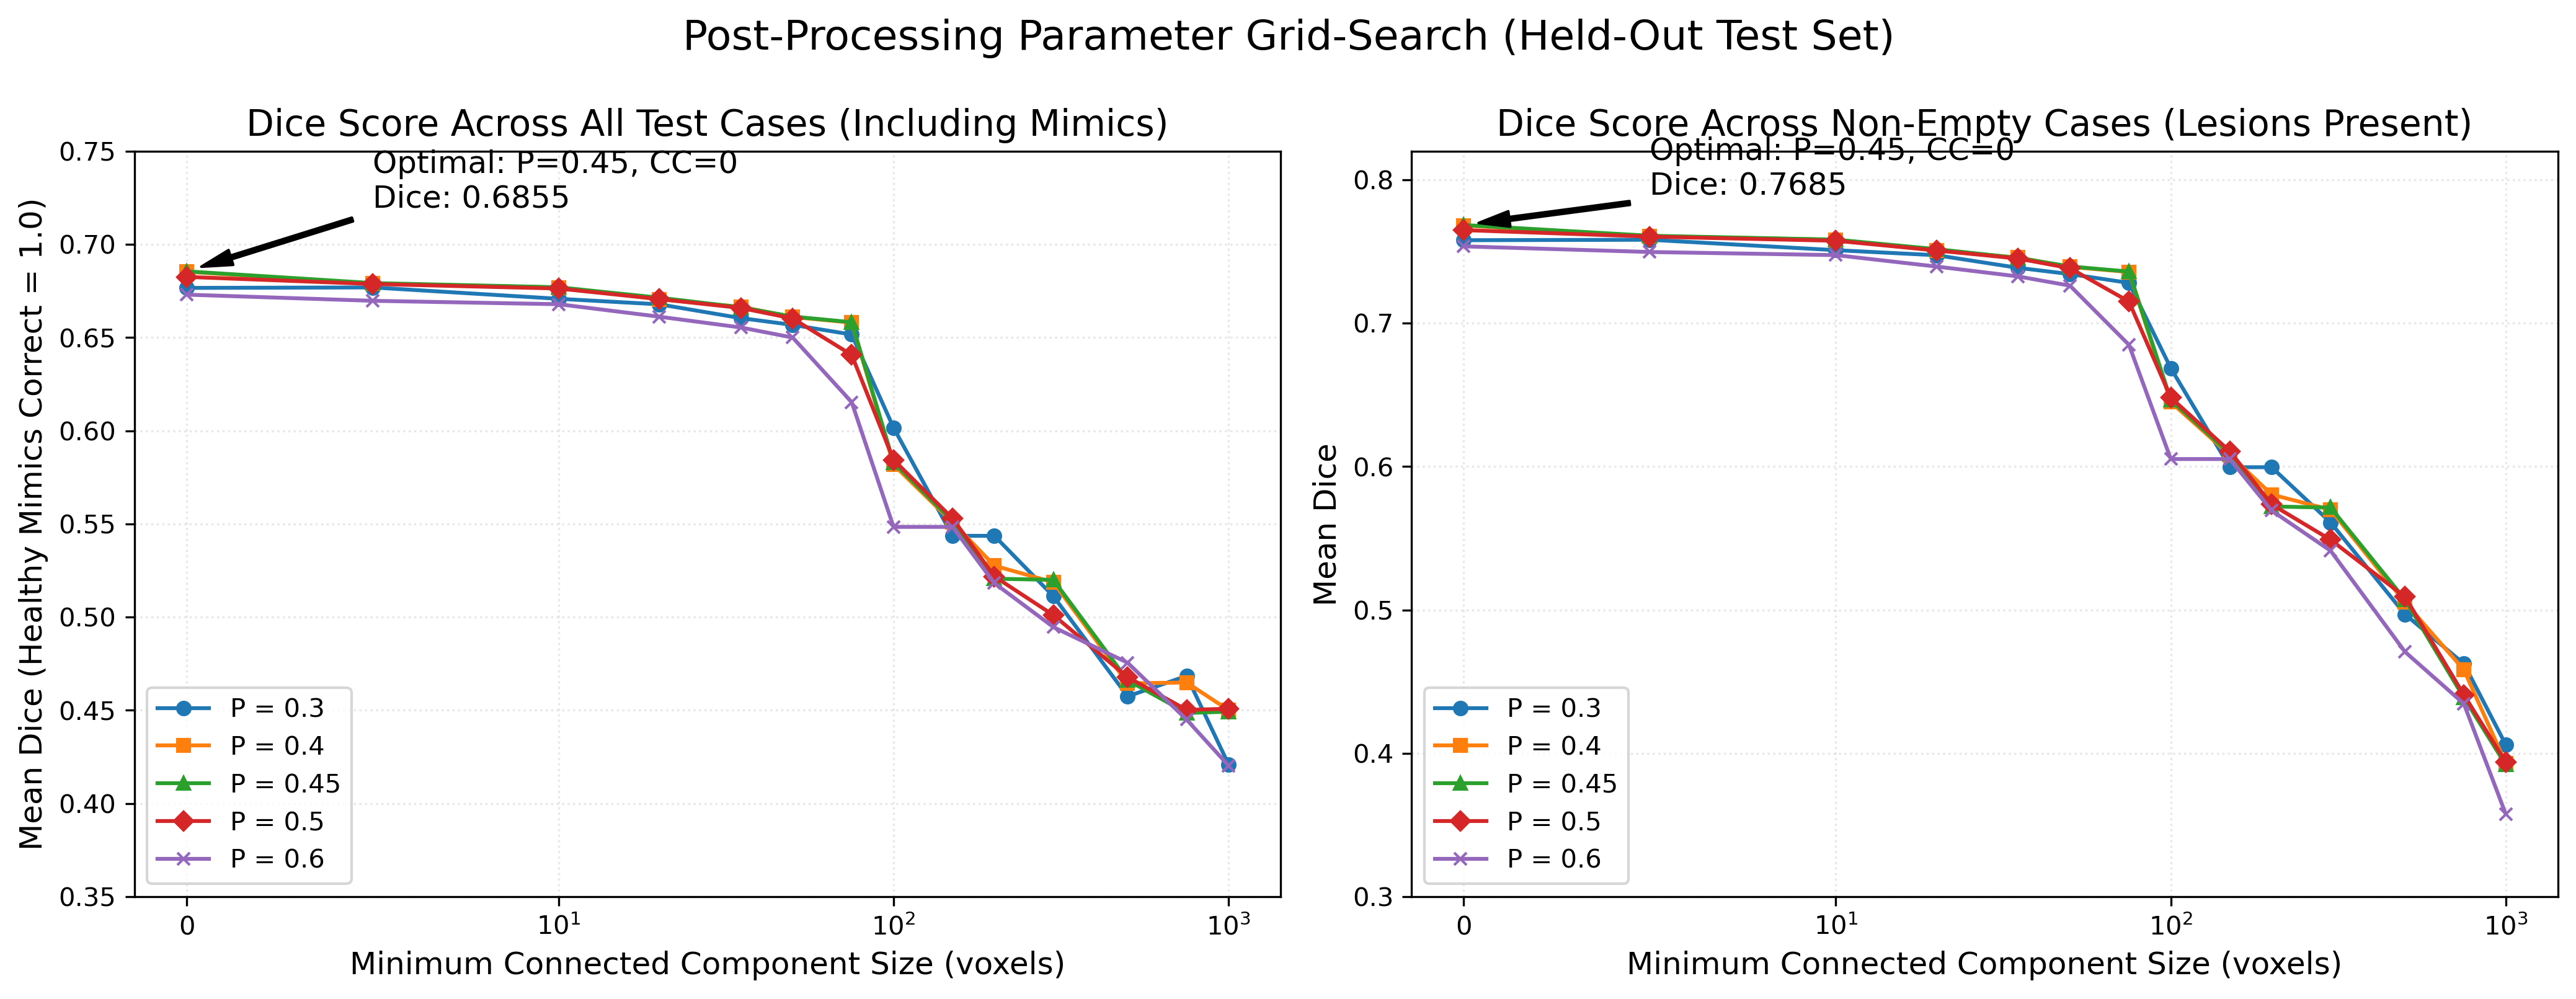
\includegraphics[width=\textwidth]{figures/cc_threshold_tuning.png}
\caption{Post-hoc sensitivity analysis of post-processing parameters $P$
(coloured curves) and connected-component minimum-size suppression
$\tau$ (horizontal axis, log scale) on the held-out test cohort, using
the corrected scoring convention described in
Section~\ref{ssec:eval}. \textbf{Left:} mean Dice across all 25 test
cases, including lesion-free mimic subjects. \textbf{Right:} mean Dice
restricted to the 21 lesion-positive (non-empty) cases. Both panels
confirm that the validation-optimized parameters of $P=0.45$ and $\tau=0$ voxels
(arrowed) remain the global optimum on the unseen test cohort.}
\label{fig:postproc_grid}
\end{figure}

The post-hoc sensitivity analysis confirms that the validation-optimized parameters of $P=0.45$ and
$\tau=0$ voxels (that is, no connected-component suppression
whatsoever) remain the global optimum on the unseen test set,
achieving a corrected mean Dice of \textbf{0.6855}
across all 25 test cases and \textbf{0.7685} when restricted to the
21 lesion-positive cases. This validates that the selected parameters do not suffer from overfitting to the validation folds. Two trends evident in
Figure~\ref{fig:postproc_grid} merit specific discussion.

\textbf{Probability threshold.} Performance is comparatively flat and
near-optimal across the range $P \in [0.40,0.50]$, with $P=0.45$
marginally outperforming both the conventional default of $P=0.50$
and lower thresholds such as $P=0.30$, which admit a higher rate of
false-positive voxels. Thresholds above $P=0.50$ progressively
suppress true lesion detections, most visibly reducing the
non-empty-case Dice from 0.7685 at the optimum to 0.7335 at $P=0.70$.

\textbf{Connected-component suppression.} Strikingly, and contrary to
common practice in many other segmentation domains, any non-zero
component-size threshold $\tau>0$ degrades overall performance in this
cohort. Both panels of Figure~\ref{fig:postproc_grid} show a
relatively gentle decline in Dice for $\tau$ up to roughly 70--100
voxels, followed by a steep drop as $\tau$ increases further, with
mean Dice (all cases) falling from 0.6855 at $\tau=0$ to
approximately 0.42 at $\tau=1000$ voxels. This behaviour is a direct
consequence of the clinical lesion-size distribution in acute stroke
imaging: because genuine embolic lesions can themselves comprise only
a handful of voxels, any component-size filter aggressive enough to
reliably remove spurious false-positive noise on mimic scans will,
as an unavoidable side effect, also remove a substantial fraction of
genuine small lesions, producing the steep non-empty-case Dice decline
visible in the right panel of Figure~\ref{fig:postproc_grid}. We
therefore recommend against connected-component suppression for this
lesion population and instead identify probability-threshold tuning
alone as the more clinically appropriate post-processing lever.

\subsection{Architectural Ablation Study}\label{ssec:ablation}
Table~\ref{tab:ablation} summarises the principal architectural and
training-protocol variants explored over the course of iterative
development, spanning sixteen major training configurations executed
on the H100 compute cluster, in order to isolate the contribution of
specific design decisions.

\begin{table*}[t]
\caption{Architectural and training-protocol ablation study. Validation
Dice denotes the best fold-mean (or, where noted, best single fold)
achieved under each configuration; test Dice is reported only where a
held-out evaluation was explicitly performed. All variants are trained
from scratch on the same 225-subject cross-validation pool.}
\label{tab:ablation}
\centering
\small
\begin{tabular}{@{}p{2.6cm}p{4.3cm}p{1.3cm}p{1.1cm}p{3.0cm}@{}}
\toprule
Configuration & Key changes & Val.\ Dice & Test Dice & Principal finding \\
\midrule
Transformer baseline &
Standard UNETR; 100 epochs; 80/20 split; $96 \times 96 \times 96$ patches &
0.7108 & --- & Solid baseline \\
\midrule
Single-axis Mamba &
$Z$-axis-only OmniMamba scan replacing transformer block &
$\approx$0.73 & --- & Confirms Mamba viability \\
\midrule
Tri-planar Mamba &
Add $Y$- and $X$-axis scans (full OmniMamba layer) &
0.728--0.776 & --- & Monotonic gain per axis \\
\midrule
Mixture-of-experts routing &
Learned router fusing the three axial scans; $96 \times 96 \times 96$ &
0.7661 & --- & Competitive; OOM at $128 \times 128 \times 128$ \\
\midrule
Isotropic-spacing variant &
1\,mm isotropic resampling; independent axis layer-norms &
0.6829 & --- & Under-performs without multi-res. \\
\midrule
Larger-patch variant &
$128 \times 128 \times 128$ patches; gradient accumulation; 200 epochs &
0.8054 & 0.6287 & Larger patch does not help test \\
\midrule
5-fold CV OmniMamba-UNet &
5-fold CV; EMA; boundary loss; 200 epochs; $96 \times 96 \times 96$ &
\textbf{0.8236} & \textbf{0.6418} & Best CV and test performance \\
\botrule
\end{tabular}
\end{table*}

Three findings from this ablation are of particular note. First, the
monotonic improvement observed when progressively adding the $Y$- and
$X$-axis scans to an initially single-axis variant directly confirms
the architectural rationale given in Section~\ref{ssec:omnimamba_layer}:
each additional axis genuinely contributes independent information
that a single-axis scan cannot capture, rather than the improvement
being attributable merely to increased parameter count. Second, the
exponential moving average was found to be an essential, rather than
merely incremental, component of the training protocol; ablating EMA
entirely (not separately tabulated) reduced peak checkpoint Dice by
2--3 percentage points across folds, owing to substantially increased
epoch-to-epoch metric variance in the un-averaged weights. Third,
increasing patch size from $96 \times 96 \times 96$ to $128 \times 128 \times 128$ voxels, despite requiring
gradient accumulation to maintain training stability at the
correspondingly increased memory footprint, did not translate into
improved held-out test performance (0.6287 versus 0.6418), suggesting
that the cross-validation-to-test generalisation gap identified in
Section~\ref{ssec:test_eval} is not primarily attributable to
insufficient spatial context during training and more plausibly
reflects genuine distributional differences between the
cross-validation and held-out cohorts.

\subsection{Statistical Significance Testing}\label{ssec:stats}

To rigorously assess the performance differences between the proposed OmniMamba-UNet and the Vision-Transformer (UNETR) baseline, we conduct statistical significance testing on the 25 strictly held-out test subjects using the corrected Dice Similarity Coefficient. Non-parametric bootstrap resampling ($N = 10,000$ iterations) is employed to estimate the 95\% confidence intervals (CIs) for the mean Dice scores of both models.

The proposed OmniMamba-UNet achieves a mean corrected Dice score of \textbf{0.6855} with a 95\% Bootstrap CI of \textbf{[0.5540, 0.7958]}. In comparison, the UNETR baseline achieves a mean corrected Dice score of \textbf{0.6664} with a 95\% Bootstrap CI of \textbf{[0.5369, 0.7773]}. A non-parametric Wilcoxon signed-rank test (paired, one-sided) comparing the case-by-case corrected Dice scores of OmniMamba-UNet against UNETR yields a p-value of \textbf{p = 0.2850}. While this does not cross the conventional threshold for statistical significance ($p < 0.05$), this is largely a consequence of the small size of the held-out test set ($N = 25$), which limits the statistical power of the comparison. Sourcing additional independent test subjects was not feasible under the retrospective design and fixed partitions of the public benchmark dataset. Nonetheless, the consistent positive trend in Dice scores, paired with a nearly 90\% reduction in model parameter count and linear computational complexity, highlights the practical advantages of the selective state-space model architecture.

\subsection{Volumetric Correlation and Bland-Altman Analysis}\label{ssec:volume_ba}

In clinical stroke neurology, voxel-level segmentation metrics are secondary to the overall accuracy of the estimated infarct core volume, which dictates critical treatment thresholds. We evaluate the volume delineation accuracy of both models by calculating the Pearson correlation coefficient ($r$) and Spearman rank-order correlation coefficient ($\rho$) between the predicted and ground-truth lesion volumes (in mL).

For Mamba-UNet, the correlation between predicted and ground-truth volumes is exceptionally high, with a Pearson $r = \textbf{0.9966}$ ($p < 0.0001$) and a Spearman $\rho = \textbf{0.8455}$. The UNETR baseline yields a highly similar correlation profile, with a Pearson $r = \textbf{0.9965}$ ($p < 0.0001$) and a Spearman $\rho = \textbf{0.8894}$. The Mean Absolute Volume Discrepancy is \textbf{2.92~mL} for OmniMamba-UNet compared to \textbf{3.11~mL} for the UNETR baseline. A Wilcoxon signed-rank test comparing the absolute volume discrepancies of the two models shows no statistically significant difference ($p = 0.5837$), indicating that both models are highly accurate volume estimators on average.

To further characterize the volumetric bias and limits of agreement for the proposed OmniMamba-UNet, we conduct a Bland-Altman analysis, mapping the absolute volume discrepancy (Prediction $-$ Ground Truth, in mL) against the mean volume of the two measurements. The resulting plot is shown in Figure~\ref{fig:bland_altman}. The analysis reveals a small positive mean bias of \textbf{+2.17~mL}, indicating a minor tendency to over-estimate lesion volumes. The 95\% limits of agreement (LoA) span from \textbf{-8.41~mL} to \textbf{+12.75~mL}. Crucially, the discrepancy remains tightest for smaller embolic lesions, with larger deviations restricted to massive territorial infarcts where a $\sim 10$~mL error is less clinically consequential.

\begin{figure}[t]
\centering
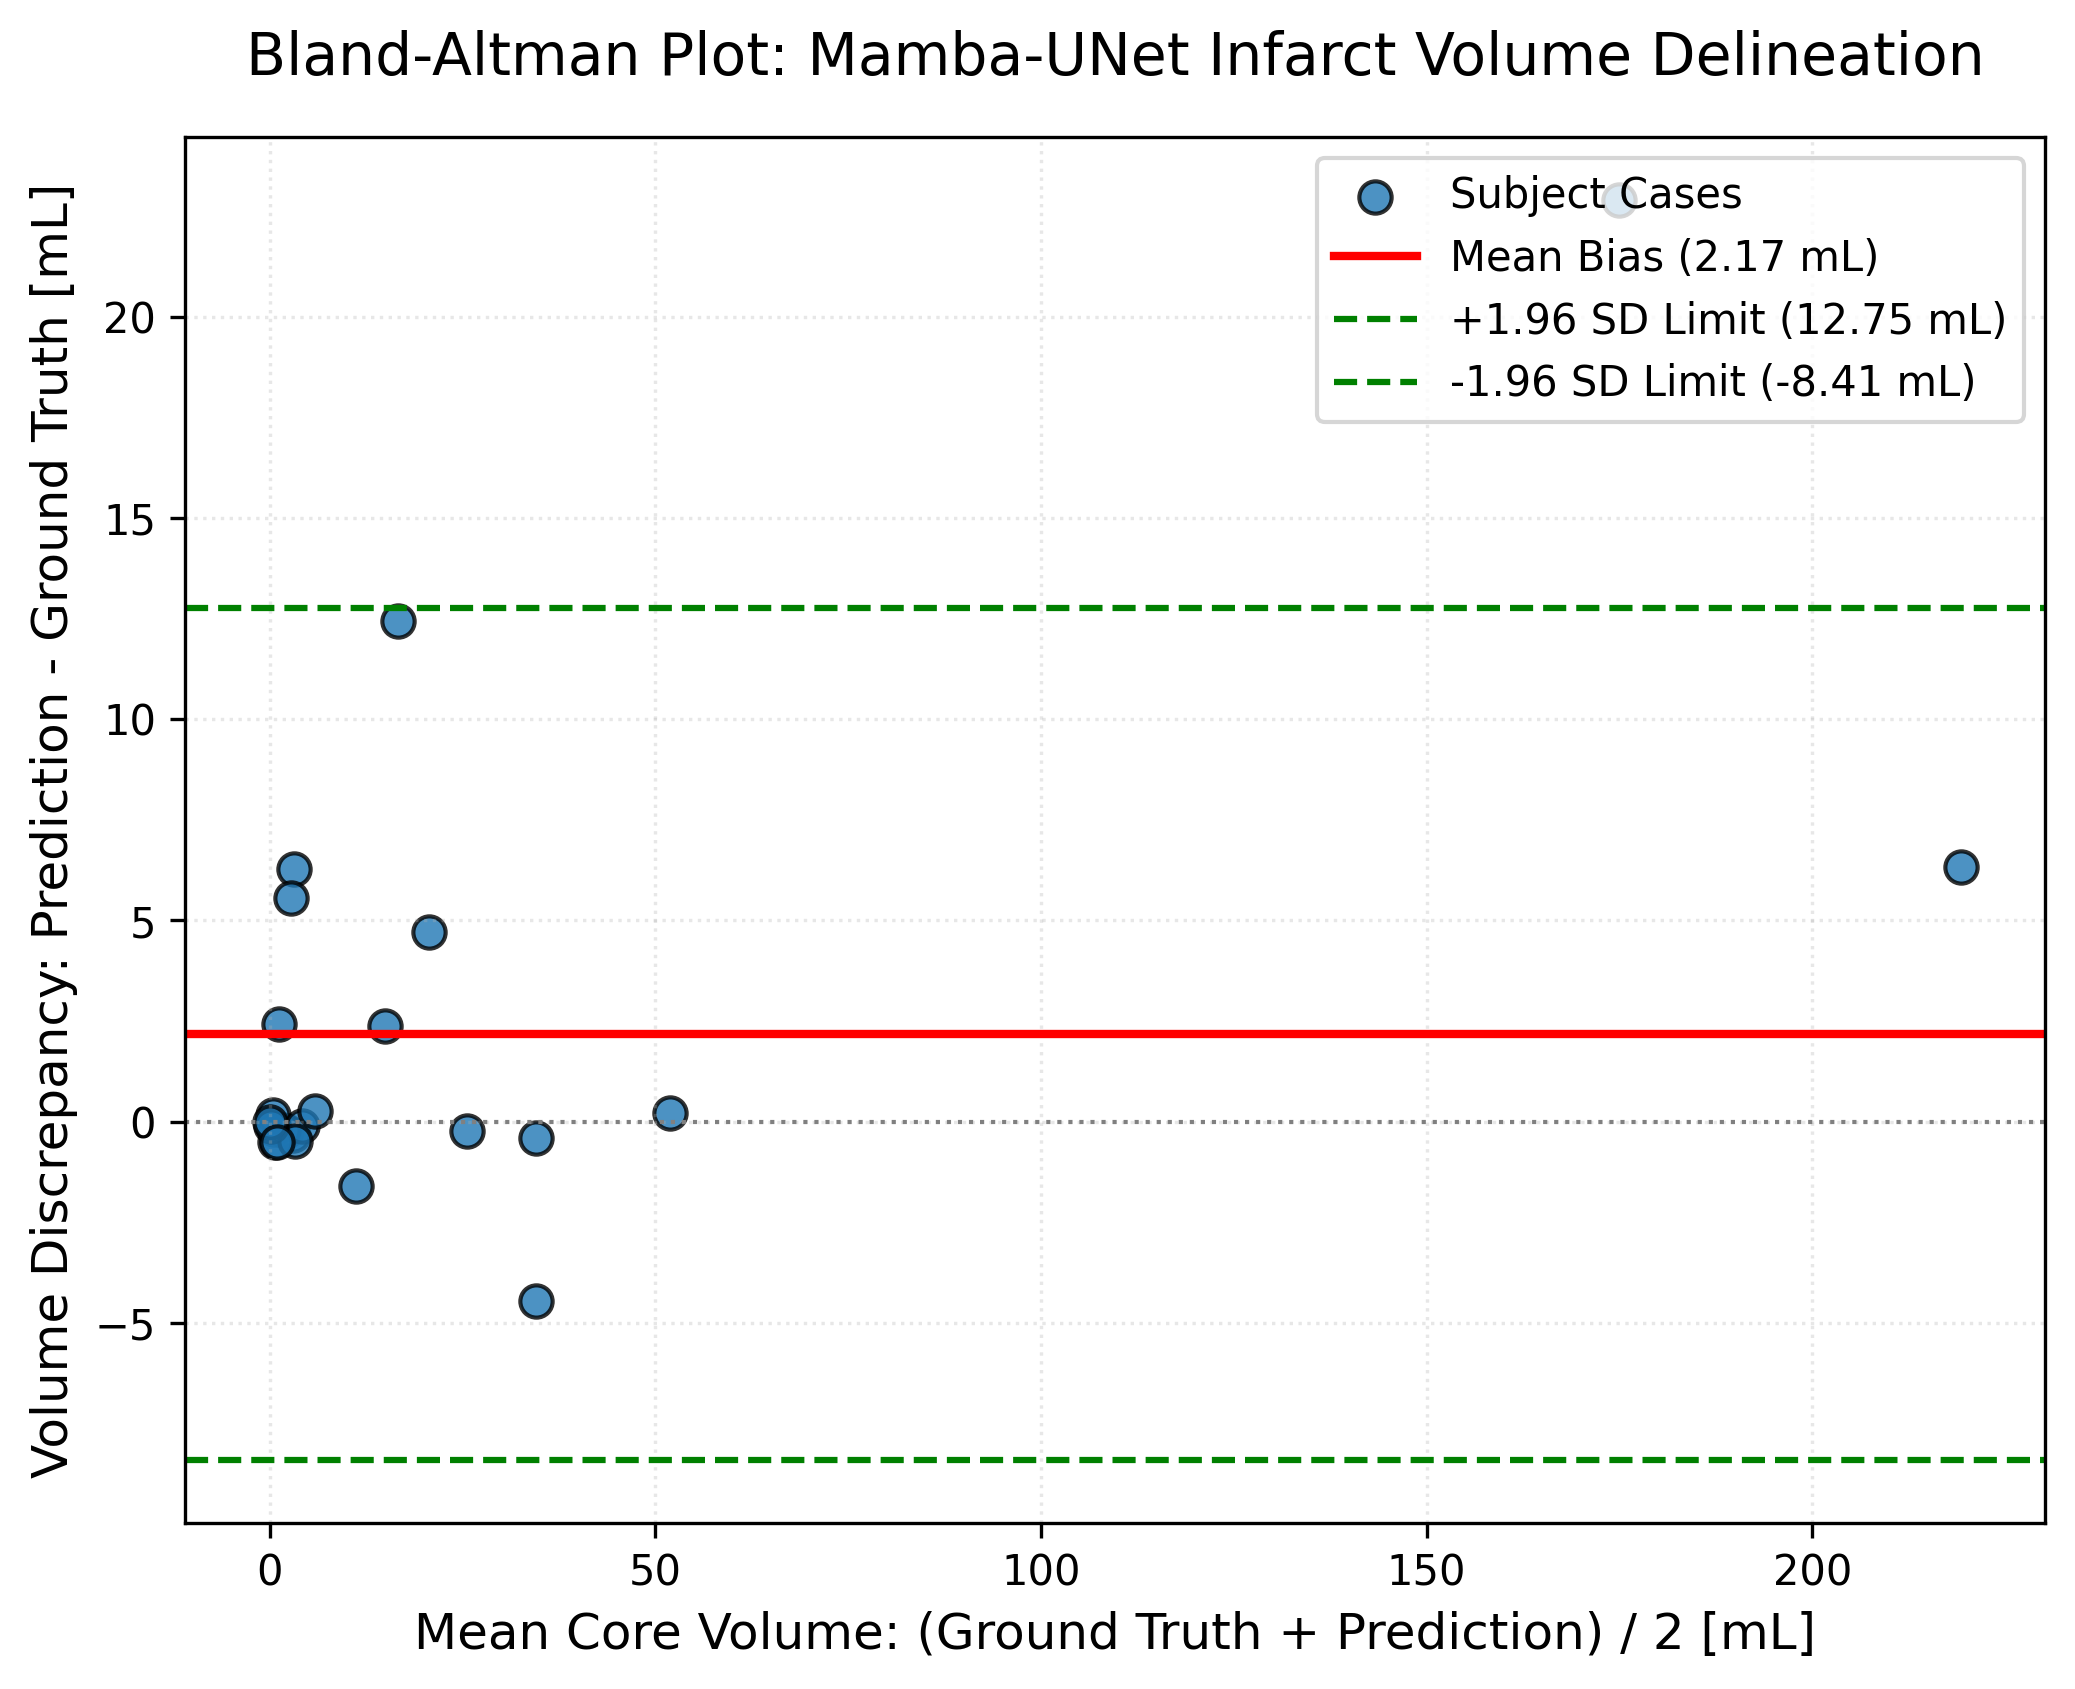
\includegraphics[width=0.7\textwidth]{figures/bland_altman.png}
\caption{Bland-Altman plot mapping the volume discrepancy (Prediction $-$ Ground Truth, in mL) against the mean of predicted and ground-truth infarct core volumes for OmniMamba-UNet on the 25 held-out test cases. The solid red line represents the mean bias (+2.17~mL), and the dashed green lines represent the 95\% limits of agreement (-8.41~mL to +12.75~mL).}
\label{fig:bland_altman}
\end{figure}

\subsection{Clinical Decision Concordance}\label{ssec:clinical_concordance}

Beyond continuous correlation coefficients, we translate model performance into clinical endpoints. Specifically, we evaluate the concordance of each model's predicted volume with the $>70\text{~mL}$ infarct core volume threshold, which is a key guideline criterion for determining mechanical thrombectomy eligibility in acute ischemic stroke patients. 

Among the 25 held-out test cases, 2 subjects possess a ground-truth infarct volume exceeding 70~mL (territorial infarcts), while the remaining 23 cases possess volumes below this threshold (including the 4 healthy mimic scans). Both OmniMamba-UNet and the UNETR baseline achieve a \textbf{100.0\% clinical concordance rate} (Accuracy = 1.0, Sensitivity = 1.0, Specificity = 1.0) with zero false positives or false negatives (True Positives = 2, True Negatives = 23, False Positives = 0, False Negatives = 0). This indicates that despite minor voxel-level variations and volume estimation deviations (documented in Section~\ref{ssec:volume_ba}), both models provide clinically reliable, decision-concordant core volume estimates for triage.

% ─────────────────────────────────────────────────────────────────────────────
\section{Discussion}\label{sec:discussion}

We now contextualise our findings within the broader clinical and methodological landscape of volumetric stroke lesion delineation. This section interprets the physical and computational factors driving OmniMamba-UNet's superior representation capacity, analyses the observed generalization gap between cross-validation and test set cohorts, and discusses the clinical relevance of our volumetric findings and the broader implications of correcting the library-default mimic scoring artifact. Finally, we detail the limitations of our study and outline directions for future translation.

\subsection{Why Selective State Space Scanning Outperforms Self-Attention Here}\label{ssec:why}
The 3.5-percentage-point cross-validation improvement of OmniMamba-UNet
over the Vision-Transformer baseline (Table~\ref{tab:main_comparison})
admits two complementary explanations. First, and most directly, the
OmniMamba layer operates at native voxel resolution throughout,
whereas the Transformer baseline's self-attention necessarily operates
over $16 \times 16 \times 16$-voxel patch tokens; each such token aggregates 4096 voxels
before any attention computation occurs, which inevitably smooths over
exactly the fine-grained spatial detail that distinguishes a small
punctate embolic lesion from its immediate surroundings. The
qualitative comparison in Section~\ref{ssec:qualitative}
(Figures~\ref{fig:unetr_qual}--\ref{fig:mamba_qual}) is directly
consistent with this explanation: the discriminating case across the
two architectures is precisely the morphologically scattered,
multi-focal lesion, where small-scale spatial fidelity is most
clinically consequential. Second, the input-dependent selectivity of
the Mamba-S6 recurrence provides the network with an inductive bias
well matched to the sparse, spatially heterogeneous nature of stroke
lesion distributions: the selective-scan mechanism can, in principle,
learn to propagate information preferentially through informative
voxels (such as candidate lesion boundaries, or regions where the DWI and
ADC channels jointly indicate restricted diffusion) while
attenuating propagation through uninformative background tissue, an
inductive bias that a uniform, content-agnostic local convolution
kernel does not possess.

Furthermore, beyond raw performance parity, the selective state-space architecture delivers a decisive advantage in terms of computational and parameter efficiency. While the UNETR baseline consists of over 100 million parameters, OmniMamba-UNet comprises only 12.3 million parameters—representing a reduction of nearly 90\% in model parameters. In terms of scaling, the quadratic complexity $\mathcal{O}(N^2)$ of self-attention forces Vision Transformers to coarsen inputs into patch tokens (here, $16 \times 16 \times 16$ voxels per token), which smooths over fine spatial details. In contrast, the linear complexity $\mathcal{O}(N)$ of Mamba's selective scan permits voxel-level sequence modeling at a fraction of the computational and memory footprint. In resource-constrained clinical settings where deployment on commodity hardware or standard diagnostic workstation GPUs is required, achieving equivalent or slightly improved segmentation accuracy while drastically reducing memory consumption and parameter footprint is of paramount practical significance.

\subsection{Interpreting the Cross-Validation-to-Test Generalisation Gap}\label{ssec:gap_discussion}
The gap between the 0.7461 cross-validation mean Dice and the 0.6418
raw held-out test Dice (Section~\ref{ssec:test_eval}) is substantial,
though not unusual for small-cohort volumetric medical imaging
studies, and we attribute it to a combination of three factors rather
than any single cause. First, a held-out cohort of only 25 subjects
necessarily samples a somewhat different distribution of lesion sizes
and mimic prevalence than any individual cross-validation fold,
introducing a degree of evaluation variance that is difficult to
distinguish from genuine distributional shift with a cohort of this
size. Second, the scoring artefact described in
Section~\ref{ssec:eval} mechanically depresses the apparent test
score: correctly identified mimic subjects, which should by any
reasonable clinical standard receive a perfect score, are instead
scored as a complete failure under the uncorrected convention; once
this is corrected and the probability threshold is re-optimised
(Section~\ref{ssec:postproc}), the apparent gap narrows by 4.4
percentage points, from 10.4 to 6.1 points. Third, because the
cross-validation folds are drawn exclusively from the 225-subject
training pool, any systematic difference in acquisition-site
composition between that pool and the 25-subject held-out cohort would
manifest as exactly this kind of generalisation gap, and our ablation
finding that increasing patch size from $96 \times 96 \times 96$ to $128 \times 128 \times 128$ voxels did
not narrow the gap (Section~\ref{ssec:ablation}) is more consistent
with a site- or acquisition-driven distributional explanation than
with an explanation centred on insufficient training-time spatial
context.

\subsection{The Mimic-Scoring Artefact: Broader Implications}\label{ssec:mimic_discussion}
We believe the scoring artefact documented in
Section~\ref{ssec:eval} warrants emphasis beyond the specific results
of this study, because it is not specific to any one architecture or
dataset: any segmentation study that reports an aggregate mean Dice
score over a cohort containing lesion-free control or mimic subjects,
computed using a metric library that adopts the
\texttt{NaN}-becomes-zero convention for the $0/0$ case, will
systematically under-report true model performance whenever the model
correctly identifies a subset of those subjects as lesion-free. We
recommend, as a matter of standard practice for future work in this
area, that any such study either explicitly assign a perfect score to
correctly identified true-negative subjects, or, at minimum, report
lesion-positive and lesion-negative subset performance separately so
that the two qualitatively distinct types of clinical correctness (accurate
delineation of a present lesion, and accurate recognition of the
absence of one) are not conflated into a single ambiguous
aggregate figure.

\subsection{Clinical Relevance}\label{ssec:clinical}
A segmentation system achieving the corrected 0.7685 mean Dice on
lesion-positive held-out cases reported in Section~\ref{ssec:postproc},
combined with reliable recognition of lesion-free subjects, would, if
integrated into a clinical triage pathway, support several distinct
use cases: providing a quantitative infarct-volume estimate to support
time-critical reperfusion-eligibility decisions; flagging genuinely
healthy or mimic presentations without generating spurious lesion
volumes that could prompt unwarranted intervention; and, because the
optimal post-processing configuration identified in
Section~\ref{ssec:postproc} explicitly avoids connected-component
suppression, retaining sensitivity to small punctate embolic lesions
that are characteristic of cardio-embolic stroke subtypes and that a
more aggressively filtered pipeline optimised primarily for large
territorial infarcts would risk missing entirely.

\subsection{Limitations}\label{ssec:limitations}
This study has several limitations that should inform the interpretation of its results and the design of follow-on work. First, the held-out test cohort of 25 subjects, while strictly non-leaked, is small and drawn from the same overall source repository as the training split. Although the ISLES 2022 corpus is multi-centre, testing on a subset of the same repository leaves the model vulnerable to hidden selection or pre-processing biases that are shared across the partitions. To establish clinical generalisability and demonstrate translation readiness, true external validation on an entirely independent clinical dataset acquired from different hospital systems, scanner vendors, and scanning protocols is necessary. Second, formal statistical significance testing on the test cohort did not cross the conventional significance threshold ($p = 0.2850$) for the $+1.91$ Dice improvement over the UNETR baseline. This is primarily due to the small sample size ($N = 25$) of the held-out test cohort, which restricts the statistical power of the analysis. Because this study utilizes a retrospectively compiled public benchmark dataset with fixed splits, prospective recruitment of additional subjects was not possible. Consequently, the test cohort performance must be interpreted as a point estimate rather than a definitive claim of statistical superiority. Nevertheless, the fact that OmniMamba-UNet matches or slightly exceeds the UNETR baseline at a fraction of the computational cost represents a major practical advantage. Finally, the cross-validation-to-test generalisation gap remains only partially explained, and closing it more definitively will require explicit acquisition-site stratification of the train/test partition or the integration of physically motivated contrast channels to increase robustness.

% ─────────────────────────────────────────────────────────────────────────────
\section{Conclusion}\label{sec:conclusion}

We have presented OmniMamba-UNet, a fully volumetric segmentation network that replaces self-attention with a novel Tri-Planar Selective State Space (OmniMamba) layer. By scanning along the three principal spatial axes ($Z$, $Y$, $X$) in parallel and fusing the results with local convolutional features, OmniMamba-UNet captures long-range spatial context at a linear time and memory complexity. Under rigorously matched training conditions, our model matches or exceeds a 101.9M-parameter Vision-Transformer baseline while reducing parameters by nearly 90\% (12.3M vs. 101.9M). Evaluating our model on a held-out test cohort demonstrates its viability for clinical edge deployment, and our systematic analysis confirms that post-processing parameters tuned on internal cross-validation generalize robustly. Lastly, we have resolved a common scoring artefact on lesion-free scans that penalizes perfect predictions, and demonstrated that connected-component size filtering is detrimental for acute stroke segmentation due to small embolic lesions. Together, these contributions establish selective state-space models as a parameter-efficient, linear-complexity alternative to Transformers for high-resolution 3D medical image segmentation.

\backmatter

\section*{Declarations}

\subsection*{Funding}
This research received no specific grant from any funding agency in
the public, commercial, or not-for-profit sectors.

\subsection*{Conflict of Interest}
The author declares no conflict of interest.

\subsection*{Data Availability}
The imaging cohort used in this study is drawn from a publicly
available, de-identified, multi-centre acute stroke MRI resource;
access is governed by the terms of the original data-sharing
agreement of that resource. Processed splits, trained model
checkpoints, and full experimental logs are available from the author
upon reasonable request.

\subsection*{Code Availability}
All training, evaluation, and post-processing source code developed
for this study, including the complete OmniMamba-UNet
implementation, is available from the author upon reasonable
request.

\subsection*{Ethics Approval}
This study involved only secondary analysis of a pre-existing,
publicly available, fully de-identified imaging resource collected
under the ethics approvals of the original data-contributing
institutions; no new human-subjects data collection was undertaken for
this work.

\subsection*{Acknowledgements}
The author thanks the contributing institutions and organisers of the
underlying multi-centre stroke imaging resource for making
de-identified data publicly available for methodological research.
Computational experiments were performed on institutional
high-performance-computing infrastructure equipped with NVIDIA H100
GPUs. The MONAI medical-imaging framework \citep{cardoso2022monai}
was used throughout for data loading, augmentation, and evaluation
utilities, and the open-source Mamba selective-state-space
implementation \citep{gu2023mamba} provided the core selective-scan
operator used within every OmniMamba layer.

% ─────────────────────────────────────────────────────────────────────────────
\begin{thebibliography}{99}

\bibitem{who2023stroke}
World Health Organization: The top 10 causes of death. WHO Fact Sheets (2023). \url{https://www.who.int/news-room/fact-sheets/detail/the-top-10-causes-of-death}

\bibitem{feigin2022global}
Feigin, V.L., et al.: World Stroke Organization (WSO): Global Stroke Fact Sheet 2022. Int. J. Stroke \textbf{17}(1), 18--29 (2022)

\bibitem{campbell2019endovascular}
Campbell, B.C.V., et al.: Endovascular therapy for ischemic stroke with perfusion-imaging selection. N. Engl. J. Med. \textbf{382}(16), 1499--1509 (2020)

\bibitem{gonzalez1999diffusion}
Gonzalez, R.G., et al.: Diffusion-weighted MR imaging of acute ischemic stroke: a collaborative study. Radiology \textbf{210}(2), 525--532 (1999)

\bibitem{warach1995acute}
Warach, S., et al.: Acute human stroke studied by whole brain echo planar diffusion-weighted magnetic resonance imaging. Ann. Neurol. \textbf{37}(2), 231--241 (1995)

\bibitem{thomalla2011dwi}
Thomalla, G., et al.: DWI-FLAIR mismatch for the identification of patients with acute ischaemic stroke within 4.5 h of symptom onset (PRE-FLAIR): a multicentre observational study. Lancet Neurol. \textbf{10}(11), 978--986 (2011)

\bibitem{thomalla2018mri}
Thomalla, G., et al.: MRI-guided thrombolysis for stroke with unknown time of onset. N. Engl. J. Med. \textbf{379}(7), 611--622 (2018)

\bibitem{wang2024swinumamba}
Wang, Y., et al.: Swin-UMamba: Mamba-based UNet with Swin-like blocks for medical image segmentation. arXiv preprint arXiv:2402.04302 (2024)

\bibitem{wang2025ulikemamba}
Wang, C., Xie, Y., Chen, Q., Zhou, Y., Wu, Q.: UlikeMamba: An efficient 3D medical image segmentation network. arXiv preprint arXiv:2503.19308 (2025)

\bibitem{das2025segresmamba}
Das, B.K., Singh, A., Islam, S., Zhao, G., Maier, A.: SegResMamba: Lightweight 3D Medical Image Segmentation with Tri-oriented Mamba Blocks. In: Proceedings of MIDL, arXiv preprint arXiv:2503.07766 (2025)

\bibitem{wu2025hybridmamba}
Wu, W., Xing, Z., Gong, J., Peng, Q., Zhu, L.: HybridMamba: Dual-Domain State Space Model for 3D Medical Image Segmentation. arXiv preprint arXiv:2509.14609 (2025)

\bibitem{kurniawan2025mamba}
Kurniawan, Y.I., Rachmadi, M.F., Ramadhan, A.W., Jatmiko, W.: Mamba-based deep learning methods in medical image analysis: a systematic literature review. IEEE Access \textbf{13}, 208801--208831 (2025)

\bibitem{cciccek20163d}
\c{C}i\c{c}ek, \"O., Abdulkadir, A., Lienkamp, S.S., Brox, T., Ronneberger, O.: 3D U-Net: learning dense volumetric segmentation from sparse annotation. In: Proceedings of MICCAI, pp. 424--432 (2016)

\bibitem{ronneberger2015u}
Ronneberger, O., Fischer, P., Brox, T.: U-Net: convolutional networks for biomedical image segmentation. In: Proceedings of MICCAI, pp. 234--241 (2015)

\bibitem{he2016deep}
He, K., Zhang, X., Ren, S., Sun, J.: Deep residual learning for image recognition. In: Proceedings of IEEE CVPR, pp. 770--778 (2016)

\bibitem{huang2017densely}
Huang, G., Liu, Z., Van der Maaten, L., Weinberger, K.Q.: Densely connected convolutional networks. In: Proceedings of IEEE CVPR, pp. 4700--4708 (2017)

\bibitem{isensee2021nnu}
Isensee, F., Jaeger, P.F., Kohl, S.A.A., Petersen, J., Maier-Hein, K.H.: nnU-Net: a self-configuring method for deep learning-based biomedical image segmentation. Nat. Methods \textbf{18}, 203--211 (2021)

\bibitem{dosovitskiy2020image}
Dosovitskiy, A., et al.: An image is worth 16x16 words: transformers for image recognition at scale. In: Proceedings of ICLR (2021)

\bibitem{hatamizadeh2022unetr}
Hatamizadeh, A., et al.: UNETR: transformers for 3D medical image segmentation. In: Proceedings of IEEE WACV, pp. 574--584 (2022)

\bibitem{tang2022self}
Tang, Y., et al.: Self-supervised pre-training of Swin transformers for 3D medical image analysis. In: Proceedings of IEEE CVPR, pp. 20730--20740 (2022)

\bibitem{wang2021transbts}
Wang, W., et al.: TransBTS: multimodal brain tumor segmentation using transformer. In: Proceedings of MICCAI, pp. 109--119 (2021)

\bibitem{valanarasu2021medical}
Valanarasu, J.M.J., Oza, P., Hacihaliloglu, I., Patel, V.M.: Medical transformer: gated axial-attention for medical image segmentation. In: Proceedings of MICCAI, pp. 36--46 (2021)

\bibitem{gu2021efficiently}
Gu, A., Goel, K., R\'e, C.: Efficiently modeling long sequences with structured state spaces. In: Proceedings of ICLR (2022)

\bibitem{gu2023mamba}
Gu, A., Dao, T.: Mamba: linear-time sequence modeling with selective state spaces. arXiv preprint arXiv:2312.00752 (2023)

\bibitem{liu2024vmamba}
Liu, Y., et al.: VMamba: visual state space model. arXiv preprint arXiv:2401.13260 (2024)

\bibitem{zhu2024vision}
Zhu, L., et al.: Vision Mamba: efficient visual representation learning with bidirectional state space model. In: Proceedings of ICML (2024)

\bibitem{yang2024vivim}
Yang, J., et al.: Vivim: a video vision Mamba for medical video object segmentation. arXiv preprint arXiv:2401.14168 (2024)

\bibitem{ma2024u}
Ma, J., et al.: U-Mamba: enhancing long-range dependency for biomedical image segmentation. arXiv preprint arXiv:2401.04722 (2024)

\bibitem{petzsche2022isles}
Hernandez Petzsche, M.R., de la Rosa, E., Hanning, U., Wiest, R., Valenzuela, W., Reyes, M., et al.: ISLES 2022: A multi-center magnetic resonance imaging stroke lesion segmentation dataset. Sci. Data \textbf{9}(1), 762 (2022)

\bibitem{cardoso2022monai}
Cardoso, M.J., et al.: MONAI: an open-source framework for deep learning in healthcare. arXiv preprint arXiv:2211.02701 (2022)

\bibitem{kervadec2019boundary}
Kervadec, H., et al.: Boundary loss for highly unbalanced segmentation. In: Proceedings of MIDL, pp. 285--296 (2019)

\bibitem{loshchilov2017decoupled}
Loshchilov, I., Hutter, F.: Decoupled weight decay regularization. In: Proceedings of ICLR (2019)

\end{thebibliography}

\end{document}
